% ==============================================================================
% Project: Digital Twin-Based Early Warning System for Cold Chain Disruption
%          Detection Using Anomaly Detection (Topic 21)
% Author: Krishna Sikheriya (Roll No.: IIT2023139), 7th Sem B.Tech (IT)
% Institution: Indian Institute of Information Technology Allahabad (IIITA)
% Instructor: Netranand Pathak
% Subject: Managing Corporate Entrepreneurship
% Recommended Compilers in Overleaf: pdfLaTeX / LuaLaTeX / XeLaTeX
% ==============================================================================

\documentclass[11pt,a4paper,oneside]{report}

% ------------------------------------------------------------------------------
% 0. COLOR PALETTE (Load xcolor FIRST with table options to prevent option clash)
% ------------------------------------------------------------------------------
\usepackage[table,xcdraw,dvipsnames]{xcolor}
\definecolor{NavyBlue}{RGB}{14, 38, 77}       % #0E264D (Primary Header & Branding)
\definecolor{AcademicBlue}{RGB}{2, 132, 199}   % #0284C7 (Accent Blue)
\definecolor{DarkSlate}{RGB}{30, 41, 59}       % #1E293B (Body Text Dark)
\definecolor{LightBlueBg}{RGB}{240, 247, 255}  % #F0F7FF (Box Fill)
\definecolor{BorderGray}{RGB}{203, 213, 225}   % #CBD5E1 (Rules & Borders)
\definecolor{HeaderGray}{RGB}{248, 250, 252}   % #F8FAFC (Table Headers)
\definecolor{HighlightRow}{RGB}{224, 242, 254} % #E0F2FE (Top-Rank Highlight)
\definecolor{EmeraldGreen}{RGB}{22, 163, 74}   % #16A34A (Positive/Verified)
\definecolor{AmberWarning}{RGB}{217, 119, 6}   % #D97706 (Limitation/Caution)
\definecolor{CrimsonRed}{RGB}{220, 38, 38}     % #DC2626 (Rejected/Failure)
\definecolor{IceTeal}{RGB}{13, 148, 136}       % #0D9488 (Cold-chain accent)

% ------------------------------------------------------------------------------
% 1. GEOMETRY & MARGINS
% ------------------------------------------------------------------------------
\usepackage[
    a4paper,
    top=2.6cm,
    bottom=2.6cm,
    left=2.8cm,
    right=2.6cm,
    headheight=16pt,
    headsep=0.8cm,
    footskip=1.2cm
]{geometry}

% ------------------------------------------------------------------------------
% 2. ENCODING & TYPOGRAPHY (Multi-Engine: pdfLaTeX / LuaLaTeX / XeLaTeX)
% ------------------------------------------------------------------------------
\usepackage{iftex}
\ifpdftex
    \usepackage[T1]{fontenc}
    \usepackage[utf8]{inputenc}
    \usepackage{mathptmx}
    \usepackage[scaled=0.92]{helvet}
    \usepackage{courier}
\else
    \usepackage{fontspec}
    \setmainfont{TeX Gyre Termes}
    \setsansfont{TeX Gyre Heros}[Scale=0.94]
    \setmonofont{TeX Gyre Cursor}[Scale=0.92]
\fi

\usepackage{microtype}
\usepackage{setspace}
\setstretch{1.14}
\setlength{\parskip}{5pt plus 2pt minus 1pt}
\setlength{\parindent}{0pt}
\setlength{\emergencystretch}{4em}
\tolerance=1200
\hbadness=2000
\usepackage{enumitem}
\usepackage{etoolbox}
\usepackage{csquotes}

% ------------------------------------------------------------------------------
% 3. MATHEMATICS & FORMULAS
% ------------------------------------------------------------------------------
\usepackage{amsmath,mathtools}
\ifpdftex
    % mathptmx provides math symbols; avoids \Bbbk clash
\else
    \usepackage{amssymb}
\fi
\usepackage{siunitx}
\sisetup{group-separator={,}, group-minimum-digits=4}

% ------------------------------------------------------------------------------
% 4. GRAPHICS & FIGURES
% ------------------------------------------------------------------------------
\usepackage{graphicx}
\usepackage{float}
\usepackage{subcaption}
\usepackage{caption}
\captionsetup{
    font={small,rm},
    labelfont={bf,color=NavyBlue},
    labelsep=colon,
    skip=8pt,
    width=0.95\textwidth
}

% ------------------------------------------------------------------------------
% 5. TABLES
% ------------------------------------------------------------------------------
\usepackage{booktabs}
\usepackage{tabularx}
\usepackage{xltabular}
\usepackage{array}
\usepackage{makecell}
\usepackage{multirow}
\newcolumntype{L}[1]{>{\raggedright\arraybackslash}p{#1}}
\newcolumntype{C}[1]{>{\centering\arraybackslash}p{#1}}
\newcolumntype{R}[1]{>{\raggedleft\arraybackslash}p{#1}}
\newcolumntype{Y}{>{\raggedright\arraybackslash}X}
\newcolumntype{Z}{>{\centering\arraybackslash}X}

% ------------------------------------------------------------------------------
% 6. CALLOUT BOXES (TCOLORBOX)
% ------------------------------------------------------------------------------
\usepackage[most]{tcolorbox}
\tcbuselibrary{skins,breakable}

% Key Finding Box
\newtcolorbox{keyfinding}[1][]{
    enhanced,
    colback=LightBlueBg,
    colframe=AcademicBlue,
    arc=4pt,
    boxrule=1.2pt,
    leftrule=5pt,
    fonttitle=\bfseries\color{NavyBlue}\sffamily,
    coltitle=NavyBlue,
    title={\large\textbf{Key Finding}\ifstrempty{#1}{}{: #1}},
    boxsep=5pt,
    left=10pt,
    right=10pt,
    top=8pt,
    bottom=8pt,
    breakable,
    shadow={1.5pt}{-1.5pt}{0pt}{black!10}
}

% Research Question Box
\newtcolorbox{researchquestion}[1][]{
    enhanced,
    colback=white,
    colframe=NavyBlue,
    arc=3pt,
    boxrule=1pt,
    leftrule=4pt,
    fonttitle=\bfseries\color{NavyBlue}\sffamily,
    coltitle=NavyBlue,
    title={\textbf{Research Question}\ifstrempty{#1}{}{: #1}},
    boxsep=4pt,
    left=8pt,
    right=8pt,
    top=6pt,
    bottom=6pt,
    breakable
}

% Methodological Decision Box
\newtcolorbox{methodologydecision}[1][]{
    enhanced,
    colback=HeaderGray,
    colframe=NavyBlue!80,
    arc=3pt,
    boxrule=1pt,
    leftrule=4pt,
    fonttitle=\bfseries\color{NavyBlue}\sffamily,
    coltitle=NavyBlue,
    title={\textbf{Methodological Decision Audit}\ifstrempty{#1}{}{: #1}},
    boxsep=4pt,
    left=8pt,
    right=8pt,
    top=6pt,
    bottom=6pt,
    breakable
}

% Important Limitation Box
\newtcolorbox{limitationbox}[1][]{
    enhanced,
    colback=AmberWarning!6!white,
    colframe=AmberWarning!90!black,
    arc=3pt,
    boxrule=1.2pt,
    leftrule=5pt,
    colbacktitle=AmberWarning!90!black,
    coltitle=white,
    fonttitle=\bfseries\color{white}\sffamily,
    title={\textbf{Important Methodological Limitation}\ifstrempty{#1}{}{: #1}},
    boxsep=5pt,
    left=10pt,
    right=10pt,
    top=8pt,
    bottom=8pt,
    breakable
}

% Proxy Data Notice Box (cold-chain specific: structural-proxy dataset caveat)
\newtcolorbox{proxynotice}[1][]{
    enhanced,
    colback=IceTeal!6!white,
    colframe=IceTeal!85!black,
    arc=3pt,
    boxrule=1.2pt,
    leftrule=5pt,
    colbacktitle=IceTeal!85!black,
    coltitle=white,
    fonttitle=\bfseries\color{white}\sffamily,
    title={\textbf{Structural-Proxy Data Notice}\ifstrempty{#1}{}{: #1}},
    boxsep=5pt,
    left=10pt,
    right=10pt,
    top=8pt,
    bottom=8pt,
    breakable
}

% ------------------------------------------------------------------------------
% 7. TIKZ DIAGRAMS
% ------------------------------------------------------------------------------
\usepackage{tikz}
\usetikzlibrary{shapes.geometric, arrows.meta, positioning, calc, fit, backgrounds, shadows}

% ------------------------------------------------------------------------------
% 8. HEADERS & FOOTERS (FANCYHDR)
% ------------------------------------------------------------------------------
\usepackage{fancyhdr}
\pagestyle{fancy}
\fancyhf{}
\renewcommand{\headrulewidth}{0.6pt}
\renewcommand{\headrule}{\hbox to\headwidth{\color{BorderGray}\leaders\hrule height \headrulewidth\hfill}}
\renewcommand{\chaptermark}[1]{\markboth{\thechapter.\ #1}{}}
\fancyhead[L]{\small\sffamily\color{DarkSlate}\nouppercase{\leftmark}}
\fancyhead[R]{\small\sffamily\color{AcademicBlue}\textbf{Cold Chain EWS Twin}}
\fancyfoot[C]{\small\sffamily\color{DarkSlate}\thepage}
\fancyfoot[R]{\scriptsize\sffamily\color{BorderGray!80!black}IIIT Allahabad}

\fancypagestyle{plain}{
    \fancyhf{}
    \renewcommand{\headrulewidth}{0pt}
    \fancyfoot[C]{\small\sffamily\color{DarkSlate}\thepage}
    \fancyfoot[R]{\scriptsize\sffamily\color{BorderGray!80!black}IIIT Allahabad}
}

% ------------------------------------------------------------------------------
% 9. SECTION & CHAPTER TITLES (TITLESEC)
% ------------------------------------------------------------------------------
\usepackage{titlesec}
\titleformat{\chapter}[display]
    {\normalfont\sffamily\huge\bfseries\color{NavyBlue}}
    {\large\bfseries\color{AcademicBlue}\MakeUppercase{\chaptertitlename}\ \thechapter}
    {4pt}
    {\hrule height 1.5pt\vspace{6pt}}
    [\vspace{4pt}\hrule height 0.5pt]

\titlespacing*{\chapter}{0pt}{-10pt}{20pt}

\titleformat{\section}
    {\normalfont\sffamily\Large\bfseries\color{NavyBlue}}
    {\thesection}{1em}{}

\titleformat{\subsection}
    {\normalfont\sffamily\large\bfseries\color{NavyBlue!90!black}}
    {\thesubsection}{0.8em}{}

\titleformat{\subsubsection}
    {\normalfont\sffamily\normalsize\bfseries\color{DarkSlate}}
    {\thesubsubsection}{0.6em}{}

% ------------------------------------------------------------------------------
% 10. HYPERLINKS & CROSS-REFERENCING
% ------------------------------------------------------------------------------
\usepackage{hyperref}
\hypersetup{
    colorlinks=true,
    linkcolor=NavyBlue,
    citecolor=AcademicBlue,
    filecolor=NavyBlue,
    urlcolor=AcademicBlue,
    pdfauthor={Krishna Sikheriya (IIT2023139)},
    pdftitle={Digital Twin-Based Early Warning System for Cold Chain Disruption Detection Using Anomaly Detection},
    pdfsubject={Managing Corporate Entrepreneurship -- Lab Assignment Topic 21},
    pdfkeywords={Digital Twin, Cold Chain, Anomaly Detection, Isolation Forest, LSTM Autoencoder, SimPy, Early Warning System, IIIT Allahabad}
}
\usepackage[nameinlink,capitalize,noabbrev]{cleveref}

% ------------------------------------------------------------------------------
% 11. BIBLIOGRAPHY
% ------------------------------------------------------------------------------
\usepackage[
    backend=biber,
    style=authoryear,
    sorting=nyt,
    maxcitenames=2,
    mincitenames=1,
    maxbibnames=8,
    doi=true,
    url=true,
    eprint=false,
    dashed=false
]{biblatex}
\addbibresource{references.bib}
\renewcommand*{\bibfont}{\small}

% ==============================================================================
% DOCUMENT BEGINS
% ==============================================================================
\begin{document}

% ------------------------------------------------------------------------------
% TITLE PAGE
% ------------------------------------------------------------------------------
\begin{titlepage}
    \begin{center}
        \vspace*{-1.2cm}

        % Institution Logo
        
\includegraphics[height=2.6cm]{figures/iiit_allahabad_logo.png}

        \vspace{0.4cm}
        {\large\bfseries\sffamily\color{NavyBlue} INDIAN INSTITUTE OF INFORMATION TECHNOLOGY, ALLAHABAD}\\[0.2cm]
        {\small\sffamily\color{DarkSlate} Department of Information Technology}\\[0.8cm]

        % Decorative Divider
        \textcolor{IceTeal}{\rule{0.85\textwidth}{1.8pt}}\\[0.6cm]

        % Main Title
        {\LARGE\bfseries\sffamily\color{NavyBlue}\setstretch{1.32}
        Digital Twin-Based Early Warning System for\\[0.35cm]
        Cold Chain Disruption Detection\\[0.22cm]
        Using Anomaly Detection\par}
        \vspace{0.45cm}

        % Subtitle & Context
        {\large\sffamily\color{IceTeal}\textbf{Semester Course Project}}\\[0.15cm]
        {\normalsize\sffamily\color{DarkSlate} Subject: \textbf{Managing Corporate Entrepreneurship}}\\[0.15cm]
%         {\normalsize\sffamily\color{DarkSlate} Instructor: \textbf{Netranand Pathak}}\\[0.6cm]

        \textcolor{IceTeal}{\rule{0.85\textwidth}{1.8pt}}\\[1.0cm]

        % Student & Submission Details in Structured Table
        \begin{tabularx}{0.88\textwidth}{r l}
            \textbf{\sffamily Prepared by:} & \sffamily Krishna Sikheriya \\
            \textbf{\sffamily Roll Number:} & \sffamily IIT2023139 \\
            \textbf{\sffamily Academic Programme:} & \sffamily B.Tech (Information Technology) --- 7th Semester \\
            \textbf{\sffamily Institution:} & \sffamily Indian Institute of Information Technology, Allahabad \\
            \textbf{\sffamily Academic Year:} & \sffamily 2026--27 \\
            \textbf{\sffamily Submission Date:} & \sffamily \rule{3.5cm}{0.4pt} \\
        \end{tabularx}

        \vspace{1.0cm}

        \begin{tcolorbox}[
            enhanced, colback=LightBlueBg, colframe=IceTeal, arc=3pt, boxrule=1pt,
            width=0.9\textwidth, boxsep=6pt, left=10pt, right=10pt, top=6pt, bottom=6pt
        ]
        \centering
        \sffamily\small
        \textbf{Live Interactive Dashboard:} \url{https://coldchain-ews-twin.streamlit.app/}\\[3pt]
        \textbf{Source Code Repository:} \url{https://github.com/Krishna200608/coldchain-ews-twin}
        \end{tcolorbox}

    \end{center}
\end{titlepage}

\pagenumbering{roman}

% ------------------------------------------------------------------------------
% ABSTRACT
% ------------------------------------------------------------------------------
\chapter*{Abstract}
\addcontentsline{toc}{chapter}{Abstract}

Cold-chain monitoring literature has concentrated overwhelmingly on post-hoc spoilage prediction and reactive, fixed-threshold temperature alarms; real-time anomaly detection embedded directly inside a digital twin, capable of flagging disruptions early enough for corrective action, remains comparatively underexplored, particularly in openly reproducible, non-proprietary form. This project develops and empirically tests a digital-twin-integrated anomaly-detection system for cold-chain disruption early warning, using two complementary anomaly-detection methods (a classical Isolation Forest baseline and an LSTM-Autoencoder) wired into a SimPy-based, three-stage discrete-event digital twin (Source $\rightarrow$ Transit $\rightarrow$ Destination) that replays real IoT temperature telemetry.

Because no cold-chain-specific, publicly available, disruption-labelled telemetry dataset exists, the Kaggle \texttt{atulanandjha/temperature-readings-iot-devices} IoT sensor log (97,606 raw readings, single-room \enquote{Out}/\enquote{In} tags, irregular sampling, temperatures in the 21--51\textdegree{}C range) is used explicitly as a \textbf{structural proxy} for cold-chain telemetry: it supplies a realistic irregularly-sampled, noisy time series but is not itself a refrigerated-transport sensor network, and this limitation is stated plainly wherever the data is discussed. Because the raw stream carries no ground-truth disruption labels, a transparently documented synthetic-injection protocol seeds 30 step/drift/flatline anomalies (5 of each per series, per series pair, \texttt{RANDOM\_SEED=42}) into a chronological 70/30 train/test split; only the 6 test-side injections are used for scientifically valid performance claims, and every injected event is explicitly labelled as a synthetic stress test, never presented as a real found anomaly.

Isolation Forest and LSTM-Autoencoder are each trained and evaluated independently (the LSTM on a free-tier Google Colab T4 GPU, verified via live \texttt{nvidia-smi} capture) and then wired as live alert generators into the digital twin's Destination stage; a cross-check between the twin's live output and the batch evaluation confirms a 100\% exact match across all 30 injections. On the six scientifically valid test-side injections, results are genuinely mixed and reported honestly rather than cherry-picked: Isolation Forest gives an early warning 64 minutes ahead of irreversibility on the Out-series drift injection and 11 minutes ahead on the In-series drift injection, while the LSTM-Autoencoder is late by 14 minutes on the same Out-series drift case; neither detector improves on a naive fixed-threshold baseline for either flatline injection or either step injection. Point-wise classification metrics (precision, recall, F1, false-positive rate, AUC-PR) are reported for both detectors on both series and show a further genuine trade-off: Isolation Forest attains substantially higher recall (80.0\% Out, 91.3\% In) at the cost of a high false-positive rate (45.6\% Out, 27.0\% In), while the LSTM-Autoencoder is more conservative and precision-favouring on the In-series (13.1\% precision versus IF's 2.0\%) but detects only 20.0\% of Out-series point-wise anomalies.

Beyond its numerical findings, the project's principal contribution is a fully documented, append-only Architectural Decision (AD) log of 35 entries spanning every methodological pivot -- including a caught-and-fixed non-causal search-window bug that had originally inflated lead times by orders of magnitude, and a caught-and-fixed single-source-of-truth violation in which a hand-transcribed comparison table disagreed with, and was ultimately shown to be wrong relative to, the pipeline's own live-computed metrics -- modelling a defensible, evidence-first, zero-fabrication approach to applied anomaly-detection system design directly relevant to the risk-management and technology-adoption themes of Managing Corporate Entrepreneurship.

\textbf{Keywords:} Digital Twin, Cold Chain Logistics, Anomaly Detection, Isolation Forest, LSTM-Autoencoder, Early Warning System, Discrete-Event Simulation, SimPy, IoT Telemetry, Structural-Proxy Data, Corporate Entrepreneurship, Risk Management.

\vspace{0.3cm}
{\small\textbf{Citation Reference:} Sikheriya, K. (2026). \textit{Digital Twin-Based Early Warning System for Cold Chain Disruption Detection Using Anomaly Detection}. Lab Assignment Final Report (Topic 21), Managing Corporate Entrepreneurship, Indian Institute of Information Technology, Allahabad.}

\clearpage
\tableofcontents
\clearpage
\listoffigures
\clearpage
\listoftables

\clearpage
\pagenumbering{arabic}

% ==============================================================================
% CHAPTER 1: INTRODUCTION
% ==============================================================================
\chapter{Introduction}
\label{chap:introduction}

\section{Background}
\label{sec:background}

Cold-chain logistics -- the unbroken sequence of refrigerated storage and transport that keeps pharmaceuticals, vaccines, dairy, meat, and fresh produce within a safe temperature band from origin to point of use -- underpins food safety and public health in ways that are almost entirely invisible until they fail. A single sustained temperature excursion during transit can render an entire shipment of vaccines unusable or accelerate microbial spoilage in perishable food beyond the point of recovery, and by the time a conventional fixed-threshold alarm fires, the excursion has frequently already crossed into an irreversible state.

The dominant academic and industrial response to this problem has been twofold: (i) \emph{post-hoc spoilage prediction}, which models shelf life or quality degradation as a function of accumulated thermal exposure once the exposure has already occurred, and (ii) \emph{reactive threshold alarms}, which fire only after a sensor reading crosses a fixed temperature limit for a sustained duration. Both approaches are diagnostic rather than anticipatory: they characterise damage that has already happened, or signal a breach only once it is underway, rather than flagging the earlier, subtler precursors -- irregular sensor gaps, drifting baselines, flatlined readings -- that often precede a full-blown disruption.

Digital twin technology, which maintains a live, continuously updated virtual replica of a physical asset or process, offers a structurally different alternative: rather than waiting for a threshold breach, an anomaly-detection model can be embedded directly inside the twin's live data flow, watching for deviations from learned normal behaviour as data arrives, and raising an alert before the point of no return is reached. Recent work on maritime refrigerated containers has shown exactly this kind of hybrid digital-twin/deep-learning approach detecting equipment degradation tens of minutes ahead of a critical cargo temperature threshold, compared to reactive alarms \parencite{vuksic2026early}. This project asks whether an analogous early-warning capability can be built, transparently evaluated, and honestly reported using only open-source tools and a publicly available IoT telemetry stream as a structural stand-in for real cold-chain sensor data.

\section{Problem Statement}
\label{sec:problem_statement}

There is no publicly available, disruption-labelled, real-world cold-chain telemetry dataset suitable for benchmarking early-warning anomaly detectors: proprietary refrigerated-transport sensor logs are commercially sensitive and rarely released, while open IoT temperature datasets that do exist (such as the Kaggle stream used in this project) were collected for generic IoT device monitoring, not cold-chain surveillance, and carry no ground-truth anomaly labels of any kind.

This creates a genuine methodological problem: any project claiming to build and evaluate a cold-chain early-warning system, using only openly available data, must either (a) implicitly overstate what the data represents, presenting a generic IoT stream as if it were real refrigerated-transport telemetry, or (b) fabricate or silently patch missing ground-truth labels, or (c) transparently document both limitations and design an evaluation protocol that is scientifically honest about what it can and cannot claim. This project adopts path (c): the IoT stream is used explicitly and repeatedly labelled as a \emph{structural proxy} -- valuable for its realistic irregular sampling and sensor-level noise characteristics, but never claimed to be an actual refrigerated-transport sensor network -- and a synthetic anomaly-injection protocol with a strict, chronologically bounded train/test split is used in place of unavailable ground-truth labels, with every injected anomaly clearly flagged as a synthetic stress-test event.

\section{Motivation and Corporate Entrepreneurship Relevance}
\label{sec:motivation}

Building a defensible early-warning capability under genuine data scarcity, and being disciplined enough to report a negative or mixed result rather than a manufactured favourable one, is not merely a machine-learning exercise -- it is a case study in evidence-first decision-making under uncertainty, directly relevant to the risk-management and technology-adoption themes of Managing Corporate Entrepreneurship:

\begin{enumerate}[leftmargin=*,itemsep=4pt]
    \item \textbf{Risk Identification Under Data Scarcity:} A cold-chain operator or technology vendor evaluating whether to invest in a digital-twin early-warning system cannot wait for a large, labelled, disruption-specific dataset to become available before making a go/no-go decision. This project demonstrates a transparent, structural-proxy-based methodology for generating credible, honestly-caveated evidence in exactly this data-scarce setting.
    \item \textbf{Disciplined Methodological Auditing:} Rejecting a plausible but flawed metric or hardcoded transcription the moment empirical evidence contradicts it -- as this project's Architectural Decision log repeatedly does -- is the same evidence-first discipline that separates defensible technology adoption decisions from ones built on convenient but ungrounded assumptions.
    \item \textbf{Honest Reporting of Mixed Results:} A commercial early-warning system that only ever reports its best-case numbers cannot be trusted for high-stakes deployment decisions. This project reports every result -- including cases where a detector is outright late, or where neither detector beats a naive baseline -- because an entrepreneurial technology-adoption decision is only as good as the evidence it is based on.
\end{enumerate}

This project addresses these questions not in theoretical abstraction, but through a working, empirically audited, and publicly deployed early-warning dashboard built entirely from open-source components.

% ==============================================================================
% CHAPTER 2: LITERATURE REVIEW
% ==============================================================================
\chapter{Literature Review}
\label{chap:literature_review}

Existing research relevant to this project spans two streams that have historically developed with limited cross-pollination: (1) cold-chain-specific monitoring and disruption/anomaly detection, and (2) the general-purpose anomaly-detection methods -- Isolation Forest and LSTM-Autoencoder reconstruction -- that this project applies to that domain.

\section{Stream 1: Cold-Chain Monitoring, Digital Twins, and Reactive Alarms}
\label{sec:lit_stream1}

The dominant paradigm in deployed cold-chain monitoring remains the fixed-threshold alarm: a sensor value is compared against a static limit, and an alert fires only once that limit is breached for a sustained duration. \textcite{meng2024costeffective} exemplify this paradigm's evolution, proposing a cost-effective over-temperature alarm system for cold-chain delivery that combines a single pallet-level sensor with a box-level digital-twin temperature model, achieving a shelf-life estimation error under $\pm1.2$ days -- a meaningful improvement in \emph{prediction accuracy} at the box level, but still fundamentally a threshold-alarm architecture rather than a live, model-embedded anomaly detector.

Digital-twin integration for cold-chain logistics has progressed furthest at the platform and service-integration level. \textcite{wu2023internet} propose an Internet-of-Everything and Digital-Twin-enabled service platform for cold-chain logistics that uses deep learning for accident identification and indoor localisation, demonstrating that digital-twin infrastructure and learned anomaly detection can be combined at the operational-platform scale; however, their deep-learning component addresses staff-safety event classification rather than early, lead-time-quantified disruption warning.

The closest direct analogue to this project's research question comes from outside food cold-chain logistics: \textcite{vuksic2026early} propose a hybrid digital-twin and deep-learning framework for early anomaly detection in maritime refrigerated containers, combining a lightweight physics-based thermal digital twin with a convolutional autoencoder trained exclusively on fault-free operation, and explicitly benchmarking time-to-detection and false-positive rate against a conventional threshold alarm. Their reported median lead time of approximately 68 minutes between an autoencoder-triggered alert and a simulated critical-temperature crossing is the same order of magnitude as this project's own Isolation-Forest lead time of 64 minutes on its Out-series drift injection (\cref{chap:results}), lending independent, cross-domain plausibility to the finding that reconstruction- or isolation-based anomaly scores can out-run a fixed-threshold alarm by tens of minutes on gradual (drift-type) disruptions specifically. Their work, however, relies on a bespoke physics-based thermal model and proprietary controller-level reefer signals; this project instead uses a pure data-pipeline digital twin (no physical thermal model) replaying a publicly available, non-proprietary telemetry stream, trading physical fidelity for openness and reproducibility.

\section{Stream 2: Anomaly-Detection Methods Applied to Cold-Chain and IoT Streams}
\label{sec:lit_stream2}

The classical anomaly-detection baseline used in this project, Isolation Forest, was introduced by \textcite{liu2008isolation} as a fundamentally different approach to anomaly detection: rather than building a profile of what \enquote{normal} looks like, the algorithm explicitly isolates anomalous points via random recursive partitioning, exploiting the fact that anomalies are both rare and structurally different from the bulk of the data. Its linear time complexity and low memory footprint make it an attractive, fast, interpretable baseline -- precisely the role it plays in this project.

Within cold-chain logistics specifically, \textcite{xie2025anomaly} propose an improved Isolation Forest variant for anomaly detection in multi-sensor cold-chain-logistics data streams, using subsampling and a cross-grouping factor to overcome the standard algorithm's tendency to fall into local optima on high-dimensional sensor data; their reported average precision (0.878), recall (0.873), and F1 score (0.864) on real multi-vehicle cold-chain-logistics sensor data substantially exceed this project's own point-wise Isolation Forest precision (0.85\% Out, 2.0\% In). This gap is instructive rather than embarrassing: their evaluation labels genuine environment/node/measurement anomalies observed directly in real fleet telemetry with five co-located sensor modalities per node, whereas this project's point-wise metrics are computed against a small number of deliberately sparse, synthetically injected single-channel anomalies inside a much larger single-sensor stream -- a structurally harder and less-favourable point-wise detection setting, discussed further in \cref{chap:discussion}.

The deep-learning anomaly detector used in this project, the LSTM-Autoencoder, follows the encoder-decoder reconstruction-error paradigm introduced by \textcite{malhotra2016lstm}: an LSTM-based encoder compresses an input window to a fixed-length latent representation, a decoder reconstructs the original window from that representation, and reconstruction error at each timestep serves as the anomaly score, on the premise that a model trained only on \enquote{normal} sequences will reconstruct anomalous sequences poorly. Their original work demonstrated robustness across predictable, unpredictable, periodic, and aperiodic time series and across a wide range of sequence lengths, which motivated this project's choice of the same architecture family for a similarly noisy, irregularly sampled IoT stream.

\section{Comparative Literature Matrix}
\label{sec:lit_matrix}

\begin{table}[H]
\centering
\caption{Comparative positioning of key literature against this project.}
\label{tab:lit_matrix}
\small
\begin{tabularx}{\textwidth}{L{3.1cm} L{4.6cm} Y}
\toprule
\textbf{Author(s) \& Year} & \textbf{Methodology / Focus} & \textbf{Relevance \& Role in This Project} \\
\midrule
\textcite{vuksic2026early} & Hybrid physics-based digital twin + convolutional autoencoder for early anomaly detection; maritime refrigerated containers. & Closest cross-domain analogue; independent corroboration that early-warning lead times of tens of minutes are achievable and operationally meaningful for cold-chain-adjacent disruptions. \\
\addlinespace
\textcite{xie2025anomaly} & Improved Isolation Forest (subsampling + cross-grouping) for multi-sensor cold-chain-logistics anomaly detection; real fleet telemetry. & Domain-specific Isolation Forest benchmark; its substantially higher point-wise precision/recall (on richer, multi-sensor, real-anomaly data) contextualises this project's own point-wise metrics. \\
\addlinespace
\textcite{wu2023internet} & Internet-of-Everything + Digital Twin service platform for cold-chain logistics with deep-learning event classification. & Establishes precedent for combining digital-twin infrastructure with learned anomaly/event detection at platform scale. \\
\addlinespace
\textcite{meng2024costeffective} & Box-level digital-twin temperature model + low-cost over-temperature alarm for cold-chain delivery. & Represents the reactive-threshold-alarm paradigm this project's early-warning approach is explicitly benchmarked against. \\
\addlinespace
\textcite{liu2008isolation} & Foundational Isolation Forest algorithm: explicit isolation via random recursive partitioning. & Theoretical foundation and direct implementation basis for this project's classical anomaly-detection baseline. \\
\addlinespace
\textcite{malhotra2016lstm} & LSTM-based Encoder-Decoder (EncDec-AD) for multi-sensor anomaly detection via reconstruction error. & Theoretical foundation and direct architectural basis for this project's LSTM-Autoencoder detector. \\
\bottomrule
\end{tabularx}
\end{table}

% ==============================================================================
% CHAPTER 3: RESEARCH GAP
% ==============================================================================
\chapter{Research Gap}
\label{chap:research_gap}

A critical synthesis of the literature reveals three major unaddressed gaps:

\begin{enumerate}[leftmargin=*,itemsep=4pt]
    \item \textbf{Post-Hoc Bias in Cold-Chain Monitoring:} The deployed cold-chain monitoring literature (\cref{sec:lit_stream1}) is dominated by fixed-threshold alarms and post-hoc shelf-life/spoilage estimation. Even digital-twin-integrated approaches such as \textcite{meng2024costeffective} primarily improve the \emph{accuracy} of a threshold-triggered alarm rather than replacing the threshold paradigm with a live, continuously-scored anomaly model embedded inside the twin's data flow itself.

    \item \textbf{Domain-Specific Anomaly Detection Requires Proprietary or Inaccessible Data:} The strongest domain-specific anomaly-detection results, such as \textcite{xie2025anomaly}'s improved Isolation Forest achieving 0.86 F1 on cold-chain-logistics sensor streams, rely on proprietary, unpublished multi-vehicle fleet telemetry with five co-located sensor modalities per node. No openly reproducible cold-chain-labelled dataset exists against which an independent, non-proprietary early-warning system can be built and benchmarked end-to-end -- a gap this project addresses directly by using an open IoT stream as an explicitly labelled structural proxy, with a fully transparent, reproducible synthetic-injection evaluation protocol in place of unavailable real disruption labels.

    \item \textbf{Unaudited Evaluation Protocols for Injected-Anomaly Benchmarks:} Where synthetic or injected anomalies are used to work around missing ground-truth labels, methodological details that materially affect reported performance -- the causality of the search window used to measure lead time, whether rolling/aggregation features leak future information, whether point-wise confusion-matrix counts are computed live or hand-transcribed into documentation -- are rarely audited or documented at the level of granularity this project's Architectural Decision log provides (\cref{chap:methodological_journey}). As demonstrated in this project (\cref{chap:methodological_journey}), an unaudited evaluation script can silently inflate lead-time claims by orders of magnitude, or a hand-transcribed results table can silently disagree with the pipeline's own live-computed numbers, without either error being visible unless deliberately checked.
\end{enumerate}

% ==============================================================================
% CHAPTER 4: AIM, OBJECTIVES AND RESEARCH QUESTIONS
% ==============================================================================
\chapter[Aim, Objectives \& RQs]{Aim, Objectives and Research Questions}
\label{chap:aim_objectives}

\section{Project Aim}
\label{sec:aim}

To develop and empirically test a digital-twin-integrated anomaly-detection system that flags cold-chain disruptions early enough for corrective action, using two complementary anomaly-detection methods wired as live alert generators into a SimPy-based discrete-event digital twin, evaluated through a transparently documented synthetic-injection protocol against a publicly available IoT telemetry stream used explicitly as a structural proxy for cold-chain data.

\section{Research Objectives}
\label{sec:objectives}

\begin{enumerate}[leftmargin=*,itemsep=3pt]
    \item \textbf{Structural-Proxy Data Acquisition \& Profiling:} Acquire, profile, and honestly characterise a real IoT temperature-sensor telemetry stream as a structural proxy for cold-chain data, documenting its sampling irregularity and its divergence from true refrigeration temperature ranges.
    \item \textbf{Transparent Injection Protocol:} Design and seed a reproducible synthetic anomaly-injection protocol (step, drift, and flatline disruption types) with a strictly chronological train/test split, in place of unavailable ground-truth disruption labels.
    \item \textbf{Classical Baseline Modelling:} Train and evaluate an Isolation Forest anomaly detector on causal, trailing-window rolling features as a fast, interpretable classical baseline.
    \item \textbf{Deep-Learning Modelling Under a Hard GPU Constraint:} Train and evaluate an LSTM-Autoencoder reconstruction-error anomaly detector, kept lightweight enough to train within a free-tier Google Colab T4 GPU session, with training genuinely verified rather than assumed.
    \item \textbf{Digital-Twin Integration:} Build a SimPy-based, three-stage discrete-event digital twin (Source $\rightarrow$ Transit $\rightarrow$ Destination) that replays the real sensor stream at its true recorded cadence and wires both anomaly detectors in as live, continuously running alert generators.
    \item \textbf{Honest, Cross-Verified Evaluation:} Report early-warning lead time and point-wise classification metrics for both detectors against a naive fixed-threshold baseline, honestly, even where a detector underperforms, and cross-check the digital twin's live output against the batch evaluation pipeline to confirm the two never silently diverge.
\end{enumerate}

\section{Research Questions}
\label{sec:rqs}

\begin{researchquestion}[RQ1: Early-Warning Lead Time]
How early can an anomaly-detection model embedded in a cold-chain digital twin flag a disruption, relative to the point at which spoilage risk becomes irreversible, and how does this compare to a naive fixed-threshold alarm?
\end{researchquestion}

\begin{researchquestion}[RQ2: Classical vs.\ Deep-Learning Trade-offs]
How do a classical Isolation Forest baseline and an LSTM-Autoencoder reconstruction-error detector compare on early-warning lead time and point-wise classification accuracy (precision, recall, F1, false-positive rate, AUC-PR), and does either dominate the other across both metrics and both sensor series?
\end{researchquestion}

\begin{researchquestion}[RQ3: Live Digital-Twin Fidelity]
Does an anomaly detector wired as a live alert generator inside a discrete-event digital twin reproduce, exactly, the same alerts and lead times as the same detector evaluated in an offline batch pipeline -- or does the act of embedding a model inside a live simulation introduce silent discrepancies?
\end{researchquestion}

% ==============================================================================
% CHAPTER 5: SYSTEM ARCHITECTURE AND METHODOLOGY
% ==============================================================================
\chapter[System Architecture \& Methodology]{System Architecture and Methodology}
\label{chap:methodology}

\section{Pipeline Overview}
\label{sec:pipeline_overview}

The system operates as a linear pipeline of five stages, each verified before the next was built upon it:

\begin{itemize}[leftmargin=*,itemsep=2pt]
    \item \textbf{Stage 1 (Ingestion \& Preprocessing):} Parses the raw Kaggle telemetry stream, deduplicates, and splits it into two independent series by sensor tag.
    \item \textbf{Stage 2 (Synthetic Injection Protocol):} Seeds 30 labelled synthetic disruptions (step, drift, flatline) and computes a fixed-threshold baseline and irreversibility timestamps.
    \item \textbf{Stage 3 (Parallel Anomaly Detection):} Trains and evaluates Isolation Forest and LSTM-Autoencoder independently on a strict chronological train/test split.
    \item \textbf{Stage 4 (Comparative Evaluation):} Benchmarks both detectors against the baseline on early-warning lead time.
    \item \textbf{Stage 5 (Digital-Twin Replay):} Replays the real sensor stream through a SimPy discrete-event simulation with both detectors wired in as live monitors, and cross-checks the live output against Stage 4.
\end{itemize}

\begin{figure}[H]
    \centering
    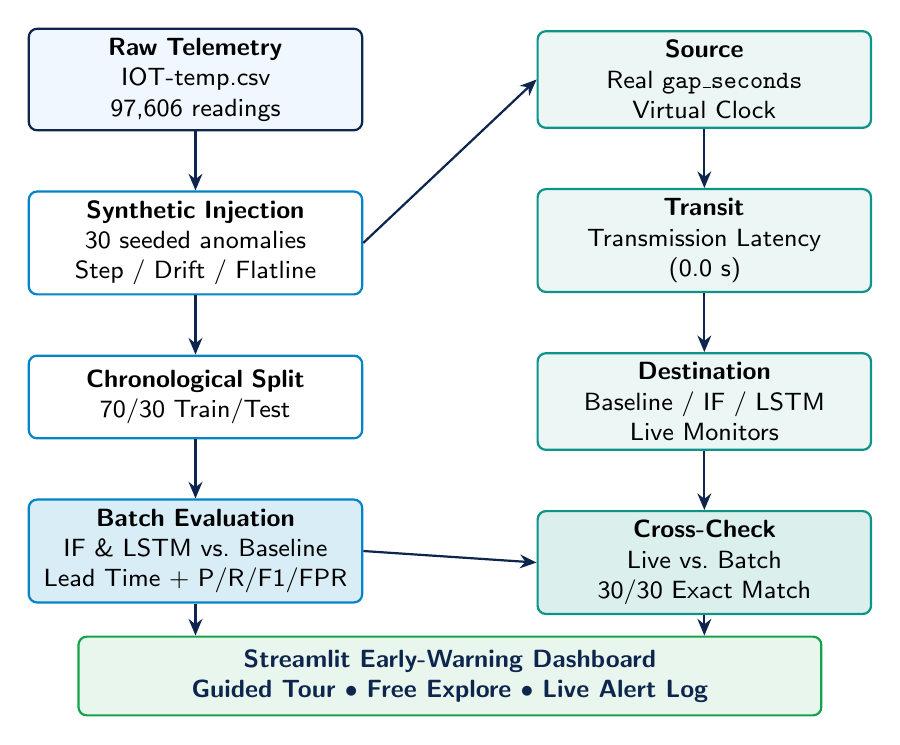
\begin{tikzpicture}[
        node distance=0.75cm and 0.7cm,
        auto,
        box/.style={
            rectangle, rounded corners=3pt, draw=NavyBlue, fill=LightBlueBg,
            thick, text width=4.0cm, minimum height=1.05cm, align=center,
            font=\small\sffamily
        },
        proc/.style={
            rectangle, rounded corners=3pt, draw=AcademicBlue, fill=white,
            thick, text width=4.0cm, minimum height=1.05cm, align=center,
            font=\small\sffamily
        },
        twinbox/.style={
            rectangle, rounded corners=3pt, draw=IceTeal, fill=IceTeal!8,
            thick, text width=4.0cm, minimum height=1.05cm, align=center,
            font=\small\sffamily
        },
        outputbox/.style={
            rectangle, rounded corners=3pt, draw=EmeraldGreen, fill=EmeraldGreen!10,
            thick, text width=9.2cm, minimum height=1.0cm, align=center,
            font=\small\sffamily\bfseries\color{NavyBlue}
        },
        arrow/.style={-{Stealth[length=6pt,width=5pt]}, thick, draw=NavyBlue}
    ]
        % Left column: offline batch pipeline
        \node[box] (raw) {\textbf{Raw Telemetry}\\IOT-temp.csv\\97,606 readings};
        \node[proc, below=of raw] (inject) {\textbf{Synthetic Injection}\\30 seeded anomalies\\Step / Drift / Flatline};
        \node[proc, below=of inject] (split) {\textbf{Chronological Split}\\70/30 Train/Test};
        \node[box, below=of split, draw=AcademicBlue, fill=AcademicBlue!15] (batch) {\textbf{Batch Evaluation}\\IF \& LSTM vs.\ Baseline\\Lead Time + P/R/F1/FPR};

        % Right column: digital twin
        \node[twinbox, right=2.2cm of raw] (source) {\textbf{Source}\\Real \texttt{gap\_seconds}\\Virtual Clock};
        \node[twinbox, below=of source] (transit) {\textbf{Transit}\\Transmission Latency\\(0.0 s)};
        \node[twinbox, below=of transit] (dest) {\textbf{Destination}\\Baseline / IF / LSTM\\Live Monitors};
        \node[box, below=of dest, draw=IceTeal, fill=IceTeal!15] (crosscheck) {\textbf{Cross-Check}\\Live vs.\ Batch\\30/30 Exact Match};

        % Synthesis
        \node[outputbox, below=1.0cm of $(batch)!0.5!(crosscheck)$] (dashboard) {
            \textbf{Streamlit Early-Warning Dashboard}\\
            Guided Tour $\bullet$ Free Explore $\bullet$ Live Alert Log
        };

        \draw[arrow] (raw) -- (inject);
        \draw[arrow] (inject) -- (split);
        \draw[arrow] (split) -- (batch);

        \draw[arrow] (source) -- (transit);
        \draw[arrow] (transit) -- (dest);
        \draw[arrow] (dest) -- (crosscheck);

        \draw[arrow] (inject.east) -- (source.west);
        \draw[arrow] (batch.east) -- (crosscheck.west);

        \draw[arrow] (batch.south) -- (batch.south |- dashboard.north);
        \draw[arrow] (crosscheck.south) -- (crosscheck.south |- dashboard.north);
    \end{tikzpicture}
    \caption{Digital-Twin-Integrated Early Warning System Architecture: the offline batch pipeline (left) trains and evaluates both detectors; the SimPy digital twin (right) replays the same stream live with both detectors wired in as monitors; a cross-check confirms the two never diverge.}
    \label{fig:system_architecture}
\end{figure}

\section{Data Source and Structural-Proxy Limitation}
\label{sec:data_source}

\begin{proxynotice}
The dataset used throughout this project, Kaggle \texttt{atulanandjha/\allowbreak temperature-readings-\allowbreak iot-devices}, is a real IoT temperature-sensor log collected for generic device monitoring. It has \textbf{no real multi-sensor spatial topology} (the \texttt{room\_id/id} field is constant, \enquote{Room Admin}, across all 97,606 readings), \textbf{no true refrigeration temperature range} (readings span 21--51\textdegree{}C, far above any real cold-chain setpoint), and \textbf{no ground-truth disruption labels of any kind}. It is used exclusively as a \textbf{structural proxy}: its irregular sampling cadence, sensor-level noise, and single-stream \enquote{Out}/\enquote{In} tag split provide a realistic substrate for building and stress-testing an anomaly-detection pipeline, but every result in this report describes performance on this proxy construct, not on real cold-chain telemetry. This caveat is repeated at every point in this report where empirical results are presented.
\end{proxynotice}

Table~\ref{tab:data_profile} summarises the dataset's key empirical properties as profiled in Milestone 1 (\texttt{docs/data\_profile.md}, \texttt{notebooks/\allowbreak 01\_eda.ipynb}).

\begin{table}[H]
\centering
\caption{Structural-Proxy Dataset Profile.}
\label{tab:data_profile}
\small
\begin{tabularx}{\textwidth}{L{4.0cm} Y}
\toprule
\textbf{Property} & \textbf{Value} \\
\midrule
Raw row count & 97,606 (1 exact duplicate row dropped $\rightarrow$ 97,605) \\
Columns & \texttt{id}, \texttt{room\_id/id} (constant \enquote{Room Admin}), \texttt{noted\_date} (requires \texttt{dayfirst=True} parsing), \texttt{temp} (integer, \textdegree{}C), \texttt{out/in} tag \\
Series split & Out = 77,261 raw / 77,260 post-split rows; In = 20,345 rows \\
Temperature range & 21--51\textdegree{}C (integer-valued) --- not a real refrigeration range \\
Sampling irregularity & Coefficient of Variation (CoV) of inter-reading gaps = 46.23, indicating strong, non-uniform sampling irregularity \\
Spatial topology & None; single constant \texttt{room\_id/id} value across the entire stream \\
Ground-truth anomaly labels & None \\
\bottomrule
\end{tabularx}
\end{table}

\begin{figure}[H]
    \centering
    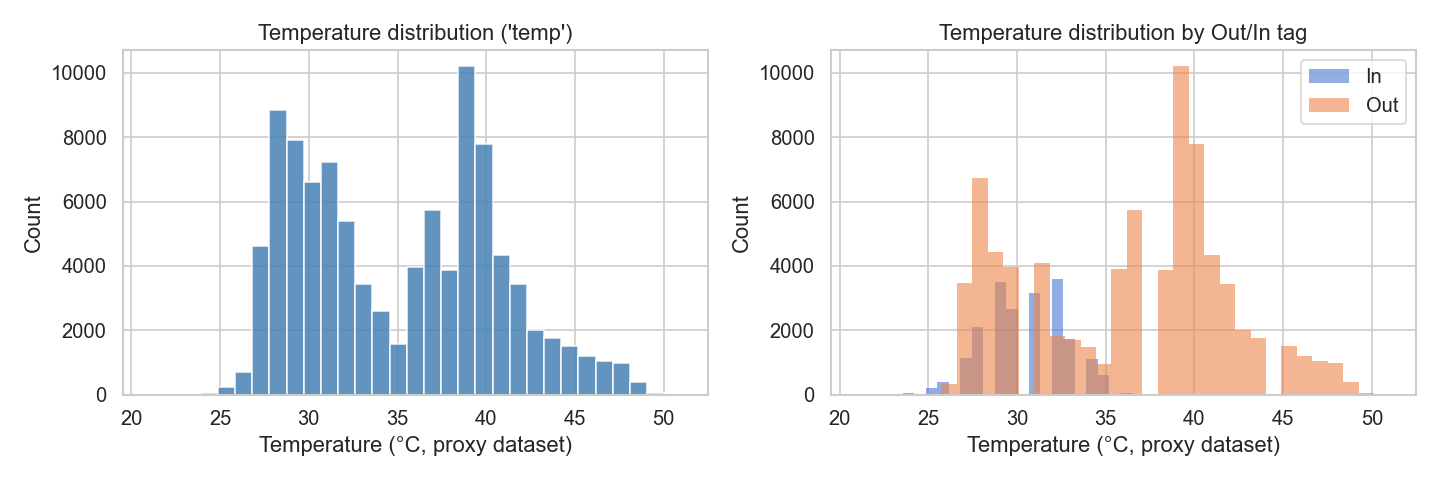
\includegraphics[width=0.92\textwidth]{figures/fig_temperature_distribution.png}
    \caption{Temperature distribution of the structural-proxy dataset, overall and by Out/In tag. The 21--51\textdegree{}C range is far outside real cold-chain setpoints, underscoring the proxy relationship to actual refrigerated-transport telemetry.}
    \label{fig:temp_distribution}
\end{figure}

\section{Stage 2: Synthetic Anomaly Injection Protocol}
\label{sec:injection_protocol}

Because the raw stream carries no ground-truth disruption labels, 30 synthetic anomalies (\texttt{RANDOM\_SEED=42}) were seeded across the two series: 5 step, 5 drift, and 5 flatline injections per series (Out and In), for $5 \times 3 \times 2 = 30$ total. A \textbf{fixed-threshold baseline} was computed as the clean-series mean plus two standard deviations (Out $= 47.6993$\textdegree{}C, In $= 34.9301$\textdegree{}C), and \textbf{irreversibility} was defined operationally as this threshold being sustained continuously for at least \texttt{D\_IRREV\_MINUTES}$=10$ minutes. Injections that straddled the chronological train/test boundary, or fell entirely on the training side, are explicitly excluded from all performance claims (\texttt{train\_or\_\allowbreak straddling\_excluded}); only the \textbf{6 test-side injections} are used for scientifically valid lead-time and point-wise metrics, listed in Table~\ref{tab:test_injections}.

\begin{table}[H]
\centering
\caption{The six test-side synthetic injections used for all performance claims.}
\label{tab:test_injections}
\small
\begin{tabular}{lll}
\toprule
\textbf{Injection ID} & \textbf{Series} & \textbf{Type} \\
\midrule
\texttt{out\_step\_001} & Out & Step \\
\texttt{out\_drift\_009} & Out & Drift \\
\texttt{out\_flatline\_012} & Out & Flatline \\
\texttt{out\_flatline\_013} & Out & Flatline \\
\texttt{in\_step\_018} & In & Step \\
\texttt{in\_drift\_023} & In & Drift \\
\bottomrule
\end{tabular}
\end{table}

\begin{methodologydecision}[Bounded Search Window]
The alarm/irreversibility search window was originally implemented \emph{unbounded} -- searching all the way to the end of each series and picking up unrelated future events. This was caught and fixed by bounding the search to \texttt{SEARCH\_HORIZON\_MINUTES=60} from injection onset, preventing artificially inflated lead-time claims (AD Log D1--D4).
\end{methodologydecision}

\begin{figure}[H]
    \centering
    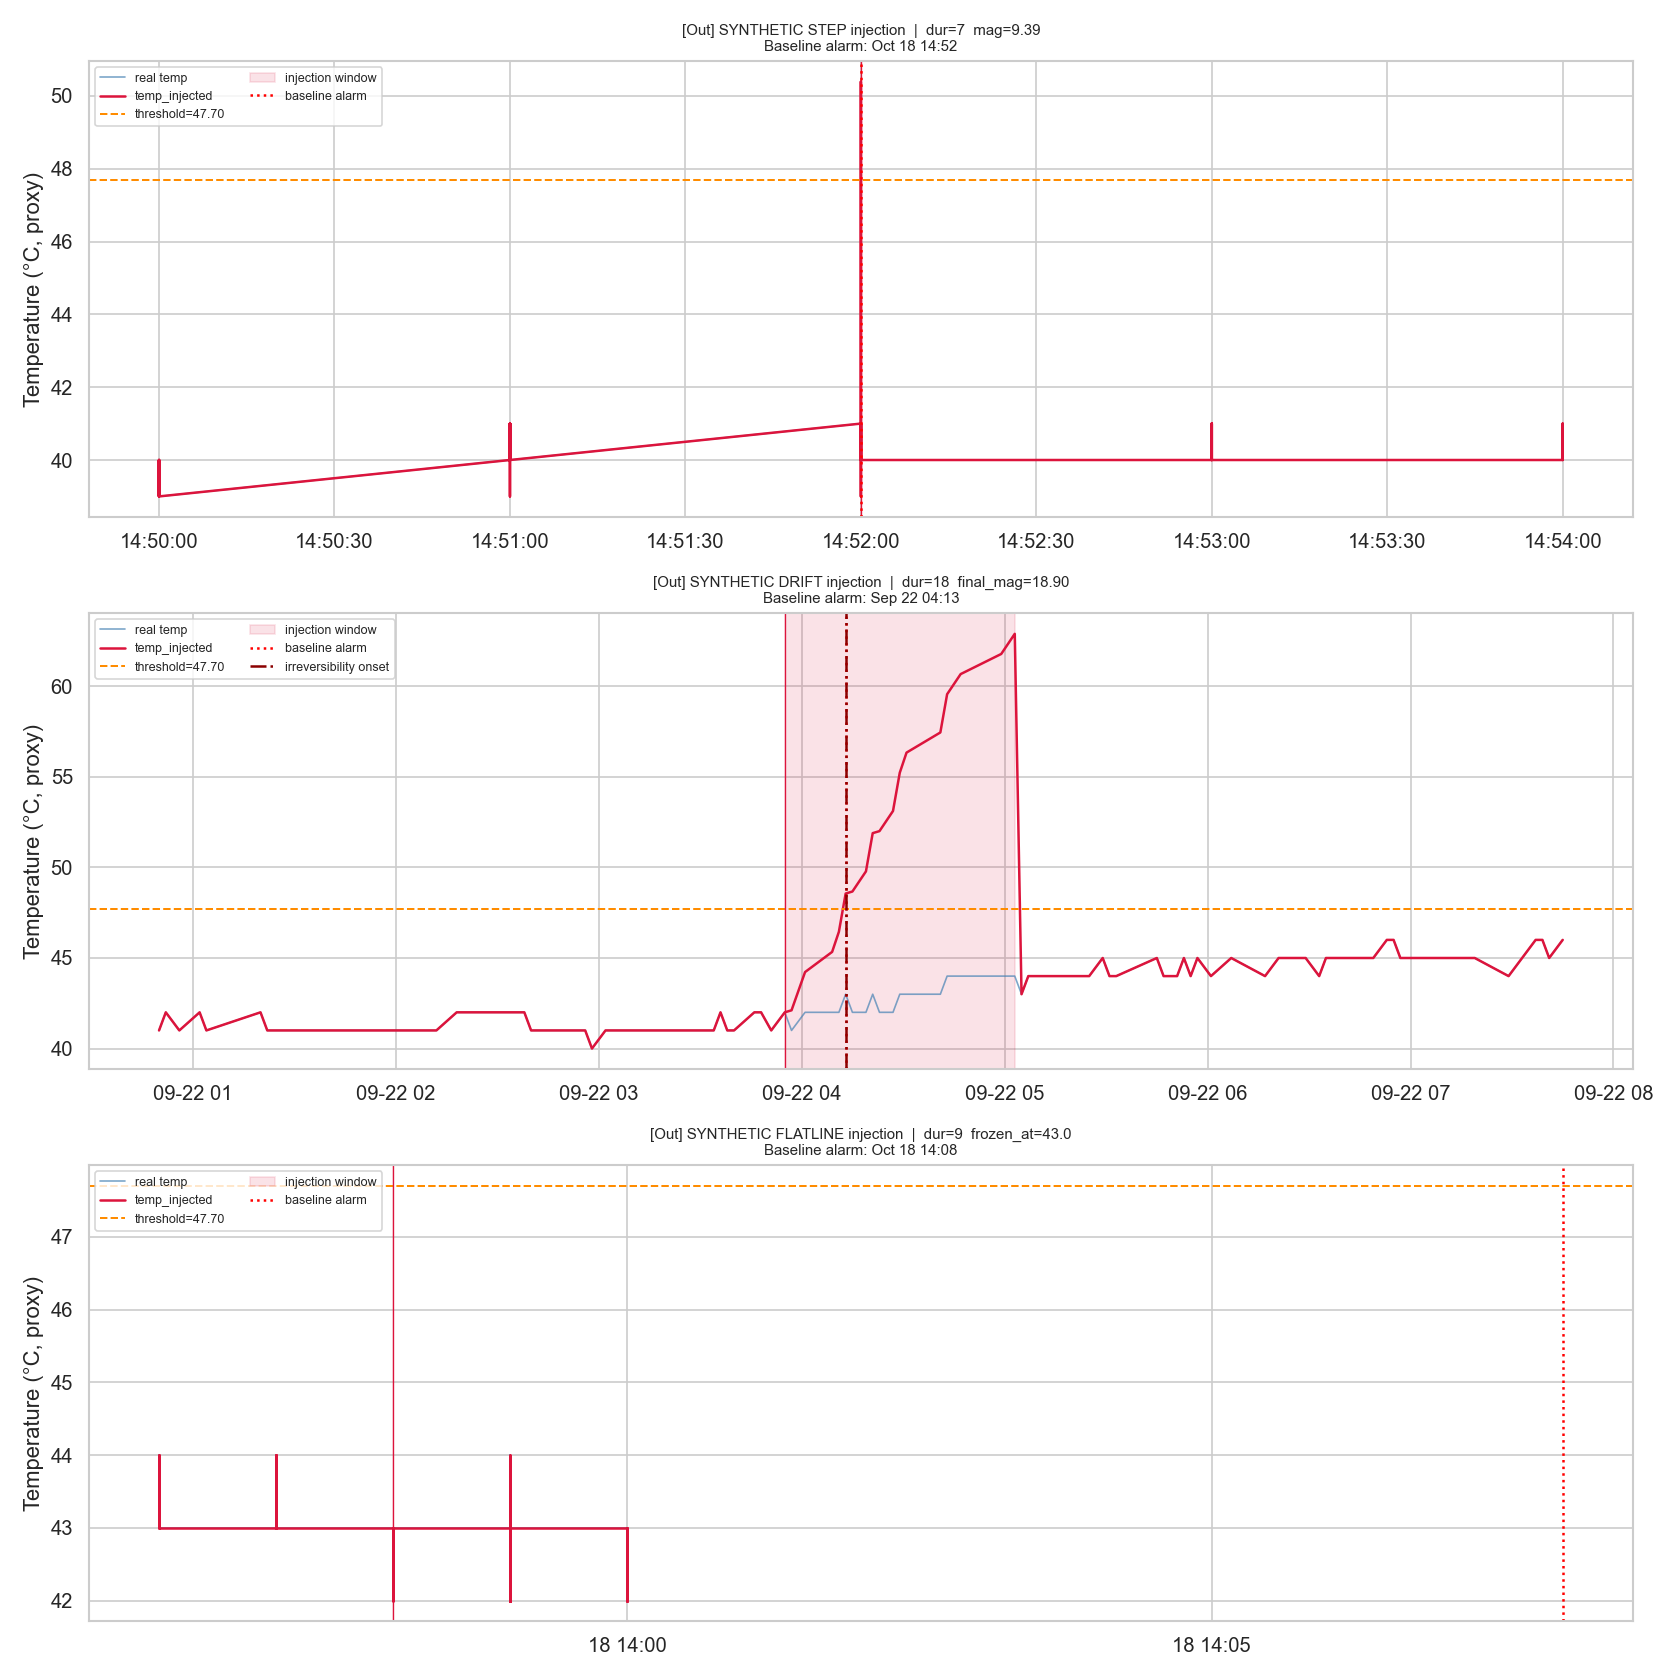
\includegraphics[width=0.92\textwidth]{figures/fig_injection_examples.png}
    \caption{Representative synthetic step, drift, and flatline injections on the Out series, explicitly labelled as synthetic stress-test events, never presented as real found anomalies.}
    \label{fig:injection_examples}
\end{figure}

\section{Stage 3a: Isolation Forest}
\label{sec:methodology_if}

Isolation Forest \parencite{liu2008isolation} isolates anomalies via recursive random partitioning rather than modelling normal behaviour explicitly. For a forest of $t$ isolation trees built on sub-samples of size $\psi$, the anomaly score for an instance $x$ is

\begin{equation}
s(x, n) = 2^{-\frac{E(h(x))}{c(n)}}
\label{eq:if_score}
\end{equation}

where $h(x)$ is the path length required to isolate $x$ in a given tree, $E(h(x))$ is its average path length across all trees, and $c(n) = 2H(n-1) - \frac{2(n-1)}{n}$ is the average path length of an unsuccessful binary search tree, used to normalise $s(x,n)$ into $[0,1]$, with values closer to 1 indicating a higher likelihood of anomaly.

\textbf{Features:} \texttt{[temp\_injected, gap\_seconds, rolling\_mean\_if, rolling\_std\_if]}, with the rolling features recomputed from the injected (not stale clean) temperature column using a causal, trailing window of length 10 -- audited in Milestone 5a (AD Log D22) and confirmed to use no \texttt{center=True} look-ahead. \textbf{Split:} chronological 70/30, cutoff \texttt{2018-10-29 11:10:47.999999}, giving Out train/test $= 63{,}887 / 13{,}372$ and In train/test $= 16{,}577 / 3{,}767$. \textbf{Hyperparameters:} \texttt{contamination='auto'} (untuned, to avoid label leakage from the synthetic injections).

\section{Stage 3b: LSTM-Autoencoder}
\label{sec:methodology_lstm}

The LSTM-Autoencoder follows the reconstruction-error paradigm of \textcite{malhotra2016lstm}: an encoder LSTM compresses an input window to a fixed-length latent vector, a \texttt{RepeatVector} layer replicates it across the output sequence length, and a decoder LSTM reconstructs the original window. The anomaly score at time $k$ is the reconstruction error of the final timestep in the causal window ending at $k$:

\begin{equation}
E(k) = \left\| x(k) - \hat{x}(k) \right\|^2
\label{eq:lstm_score}
\end{equation}

where $x(k)$ is the true feature vector at time $k$ and $\hat{x}(k)$ is the model's reconstruction of it from the window $[k-29, k]$.

\textbf{Architecture:} Encoder LSTM(32) $\rightarrow$ RepeatVector $\rightarrow$ Decoder LSTM(32) $\rightarrow$ Dense(2), deliberately kept lightweight to remain within a free-tier Google Colab T4 GPU session at every stage. \textbf{Windows:} length 30, stride 5 (training only); \textbf{features:} \texttt{[temp\_injected, log1p(gap\_seconds)]}, train-only normalised. \textbf{Scoring (AD Log D16):} causal, single-window-per-row -- the score at row $k$ uses only the window ending at $k$, never a centred or future-looking window, and the first 29 rows of each region are undefined (NaN blind spot), verified not to overlap any test-side injection onset. \textbf{Threshold (AD Log D13):} train-only mean $+\ 2\sigma$ of reconstruction error (Out $=1.010091$, In $=1.512753$).

\begin{limitationbox}[GPU Constraint]
All LSTM-Autoencoder training was constrained to a free-tier Google Colab T4 GPU session. The architecture (two 32-unit LSTM layers) was deliberately kept small enough that this was never a bottleneck; no larger architecture, batch size, or multi-GPU configuration was assumed at any point.
\end{limitationbox}

\section{Stage 4: Early-Warning Lead-Time Metric}
\label{sec:lead_time_metric}

The core research-question metric is early-warning lead time: for a given test-side injection with irreversibility onset $t_{\text{irrev}}$ and a detector alarm timestamp $t_{\text{alarm}}$ (the first timestamp within the bounded search window at which the detector's score crosses its threshold), lead time is

\begin{equation}
\Delta t_{\text{lead}} = t_{\text{irrev}} - t_{\text{alarm}}
\label{eq:lead_time}
\end{equation}

A positive $\Delta t_{\text{lead}}$ indicates the detector alarmed \emph{before} irreversibility (a genuine early warning); a negative value indicates the detector was \emph{late}; and an undefined (null) value indicates either no alarm was raised within the bounded window, or -- for flatline injections specifically -- no irreversibility timestamp was ever reached, so no lead time can be computed even where an alarm did fire.

\section{Stage 5: SimPy Digital-Twin Replay Engine}
\label{sec:digital_twin}

The digital twin is implemented as a three-stage SimPy discrete-event simulation: \textbf{Source} (replays the real sensor stream using its true recorded \texttt{gap\_seconds} as the virtual clock, not wall-clock time), \textbf{Transit} (a transmission-latency stage, \texttt{TRANSIT\_LATENCY\_SECONDS=0.0} in this configuration), and \textbf{Destination} (runs \texttt{BaselineMonitor}, \texttt{IFMonitor}, and \texttt{LSTMMonitor} live, as data arrives). The three stages are explicitly reframed as a \emph{data pipeline} (sensor generation $\rightarrow$ transmission $\rightarrow$ monitoring), not a physical spatial topology, since the source data itself carries no real multi-sensor spatial structure (\cref{sec:data_source}).

\begin{methodologydecision}[Byte-Exact Replay Verification]
Before wiring detectors into the twin, the replay engine itself was verified against the real sensor stream: byte-exact replay of all readings, zero value mismatches, and $0.00\times10^{0}$s simulated-time discrepancy across a full replay completing in 6.03 seconds of wall-clock time (AD Log D17--D19).
\end{methodologydecision}

The live monitors' buffers accumulate continuously with no resets at train/validation/test boundaries (AD Log D23), and their outputs were cross-checked against every Milestone 2--4b batch-evaluation result: a \textbf{100\% exact match} across all 30 injections $\times$ 3 detectors (baseline 30/30; Isolation Forest and LSTM 6/6 on the scientifically valid test-side injections), with the 24 train-side results correctly excluded from performance claims and retained only as demonstration material (AD Log D26). This cross-check directly answers RQ3 (\cref{sec:rqs}): the live digital twin and the offline batch pipeline never silently diverge.

% ==============================================================================
% CHAPTER 6: RESULTS AND FINDINGS
% ==============================================================================
\chapter{Results and Findings}
\label{chap:results}

\begin{proxynotice}
Every result in this chapter describes performance on the structural-proxy IoT dataset (\cref{sec:data_source}), evaluated against synthetic, explicitly labelled stress-test injections (\cref{sec:injection_protocol}). No claim in this chapter should be read as a statement about real cold-chain disruption detection performance.
\end{proxynotice}

\section{Three-Way Lead-Time Comparison: The Core Research-Question Result}
\label{sec:res_leadtime}

Table~\ref{tab:leadtime} reports early-warning lead time (\cref{eq:lead_time}) for all three detectors (fixed-threshold baseline, Isolation Forest, LSTM-Autoencoder) on all six test-side injections, exactly as computed by \texttt{src/three\_way\_comparison.py} and unaffected by the point-wise-metrics correction described in \cref{chap:methodological_journey}.

\begin{table}[H]
\centering
\caption{Early-warning lead time (minutes before irreversibility) on the six test-side injections. Positive values are an early warning; negative values indicate the detector was late; null indicates no alarm within the bounded search window, or (for flatlines) no irreversibility timestamp was ever reached.}
\label{tab:leadtime}
\small
\begin{tabular}{lccccc}
\toprule
\textbf{Injection} & \textbf{Type} & \textbf{Series} & \textbf{Baseline} & \textbf{Isolation Forest} & \textbf{LSTM-AE} \\
\midrule
\texttt{out\_step\_001} & Step & Out & 0.0 & 0.0 & 0.0 \\
\texttt{out\_drift\_009} & Drift & Out & 0.0 & \textbf{+64.0} & \textbf{$-$14.0 (late)} \\
\texttt{out\_flatline\_012} & Flatline & Out & null & null$^{\ast}$ & null$^{\ast}$ \\
\texttt{out\_flatline\_013} & Flatline & Out & null & null$^{\ast}$ & null (never alarmed) \\
\texttt{in\_step\_018} & Step & In & 0.0 & 0.0 & 0.0 \\
\texttt{in\_drift\_023} & Drift & In & 0.0 & \textbf{+11.0} & 0.0 \\
\bottomrule
\end{tabular}
\vspace{2pt}
\\{\footnotesize $^{\ast}$An alarm \emph{was} raised (IF at 21:09 on \texttt{out\_flatline\_012} and 01:22 on \texttt{out\_flatline\_013}; LSTM at 21:03 on \texttt{out\_flatline\_012}) but no irreversibility timestamp was ever reached for either flatline injection, so lead time is undefined rather than zero.}
\end{table}

\begin{figure}[H]
    \centering
    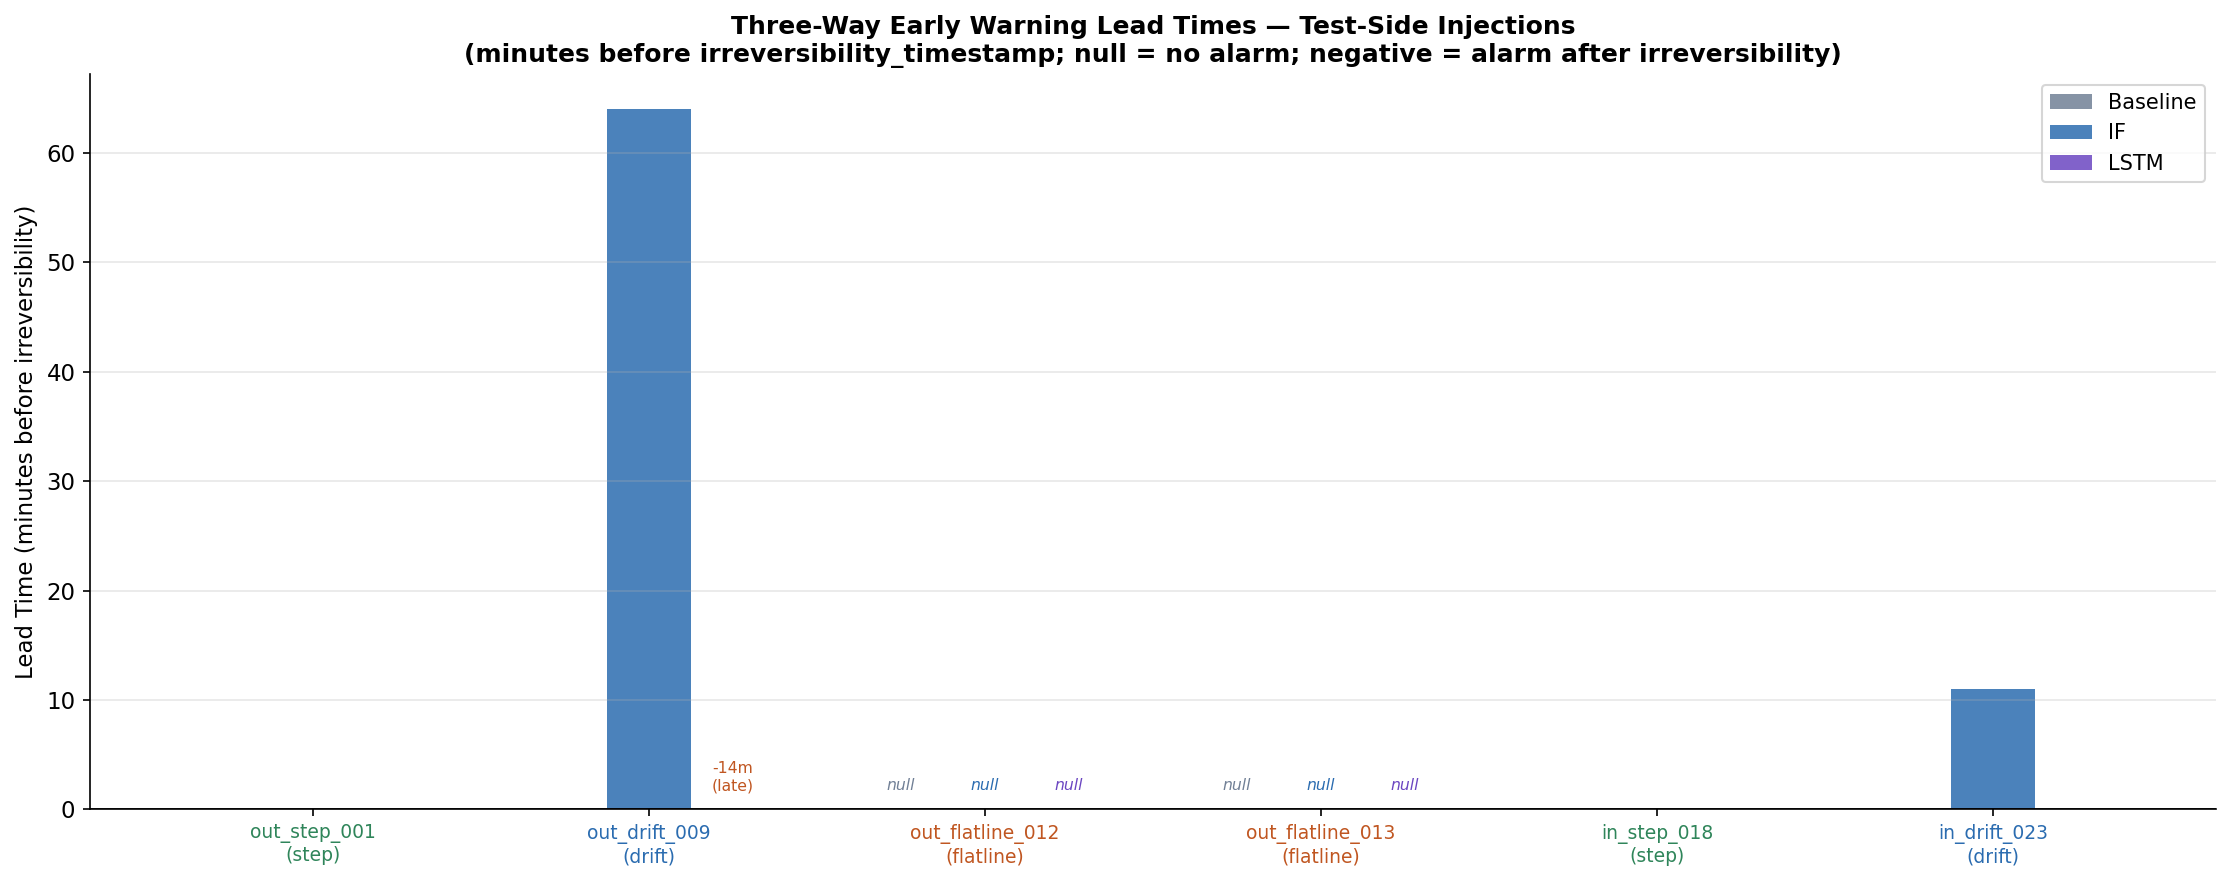
\includegraphics[width=0.95\textwidth]{figures/fig_m4b_three_way_lead_times.png}
    \caption{Early-warning lead time by detector across the six test-side injections. Isolation Forest is the only detector to beat the naive baseline, on both drift injections; neither detector improves on the baseline for either step or either flatline injection.}
    \label{fig:leadtime_chart}
\end{figure}

\begin{keyfinding}[Genuinely Mixed, Non-Cherry-Picked Result]
Isolation Forest wins decisively on drift-type early warning (+64.0 min Out, +11.0 min In), while the LSTM-Autoencoder is actually \emph{late} by 14.0 minutes on the one Out-series drift case where it does eventually alarm. Neither detector beats the naive fixed-threshold baseline on either step injection (all three detectors alarm at exactly the same timestamp, lead time 0.0) or on either flatline injection. This is reported exactly as measured, with no result omitted or adjusted.
\end{keyfinding}

\section{Point-Wise Classification Metrics}
\label{sec:res_pointwise}

Table~\ref{tab:pointwise} reports point-wise precision, recall, F1, false-positive rate, and AUC-PR for both detectors on both series, computed on the chronological test split (Out: 13,372 rows, 65 true-anomaly rows; In: 3,767 rows, 23 true-anomaly rows). These are the corrected, single-source-of-truth values described in AD Log D35 (\cref{chap:methodological_journey}); every reported precision/recall/F1/FPR pair satisfies $\text{TP}+\text{FN} = $ true-anomaly-row count exactly, verified by a permanent regression assertion in the evaluation code.

\begin{table}[H]
\centering
\caption{Point-wise classification metrics on the test split (test valid-score rows only; LSTM excludes 29 blind-spot rows per series with undefined scores).}
\label{tab:pointwise}
\small
\begin{tabular}{lrrrr}
\toprule
\textbf{Metric} & \textbf{IF --- Out} & \textbf{LSTM --- Out} & \textbf{IF --- In} & \textbf{LSTM --- In} \\
\midrule
True anomaly rows & 65 & 65 & 23 & 23 \\
TP & 52 & 13 & 21 & 16 \\
FP & 6,067 & 2,722 & 1,010 & 106 \\
TN & 7,240 & 10,556 & 2,734 & 3,609 \\
FN & 13 & 52 & 2 & 7 \\
\midrule
Precision & 0.0085 & 0.0048 & 0.0204 & 0.1311 \\
Recall & 0.8000 & 0.2000 & 0.9130 & 0.6957 \\
F1 & 0.0168 & 0.0093 & 0.0398 & 0.2207 \\
FPR & 0.4559 & 0.2050 & 0.2698 & 0.0285 \\
AUC-PR & 0.0676 & 0.0049 & 0.2371 & 0.3852 \\
\bottomrule
\end{tabular}
\end{table}

\begin{figure}[H]
    \centering
    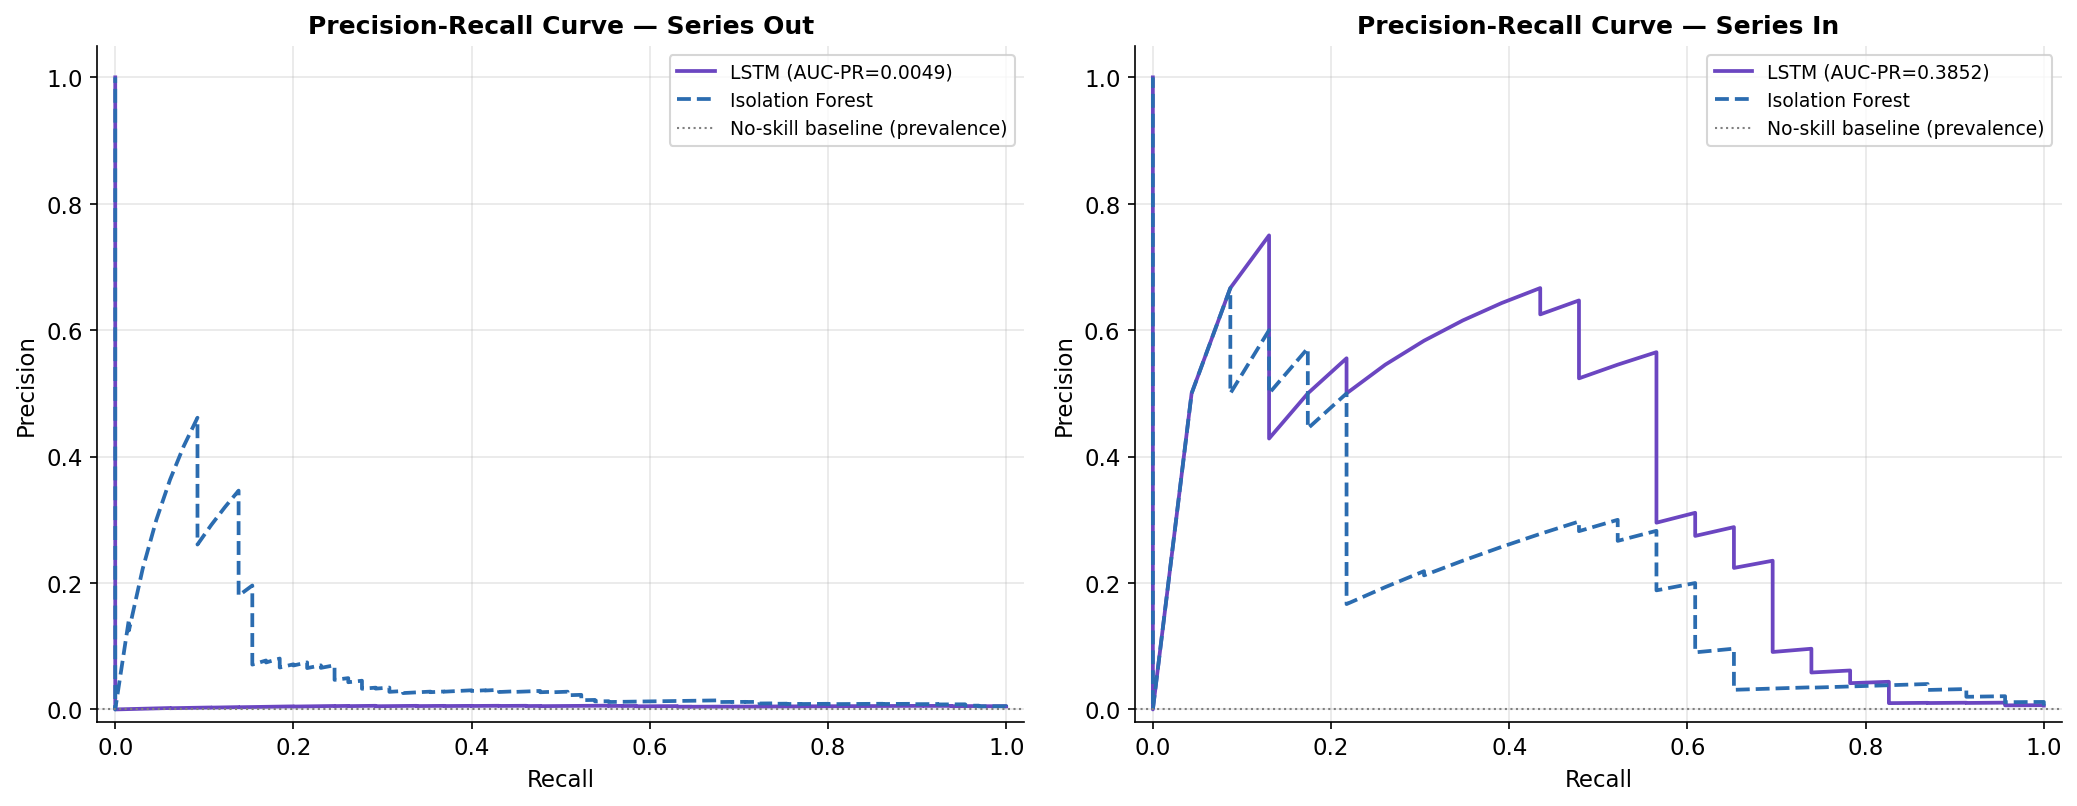
\includegraphics[width=0.95\textwidth]{figures/fig_m4b_pr_curves.png}
    \caption{Precision-recall curves, Isolation Forest vs.\ LSTM-Autoencoder, both series. The LSTM-Autoencoder dominates on the In series (AUC-PR 0.385 vs.\ 0.237) but is essentially at chance on the Out series (AUC-PR 0.005 vs.\ IF's 0.068).}
    \label{fig:pr_curves}
\end{figure}

\begin{keyfinding}[A Second Genuine Trade-off]
Isolation Forest achieves substantially higher recall on both series (80.0\% Out, 91.3\% In) at the cost of a high false-positive rate (45.6\% Out, 27.0\% In). The LSTM-Autoencoder is more conservative: on the In series it trades recall for a markedly better precision (13.1\% vs.\ IF's 2.0\%) and a much lower false-positive rate (2.9\% vs.\ 27.0\%), but on the Out series it detects only 20.0\% of point-wise anomalies and its AUC-PR (0.0049) is close to chance. Neither detector dominates the other across both series and both metric families -- consistent with, and reinforcing, the lead-time result in \cref{sec:res_leadtime}.
\end{keyfinding}

\begin{figure}[H]
    \centering
    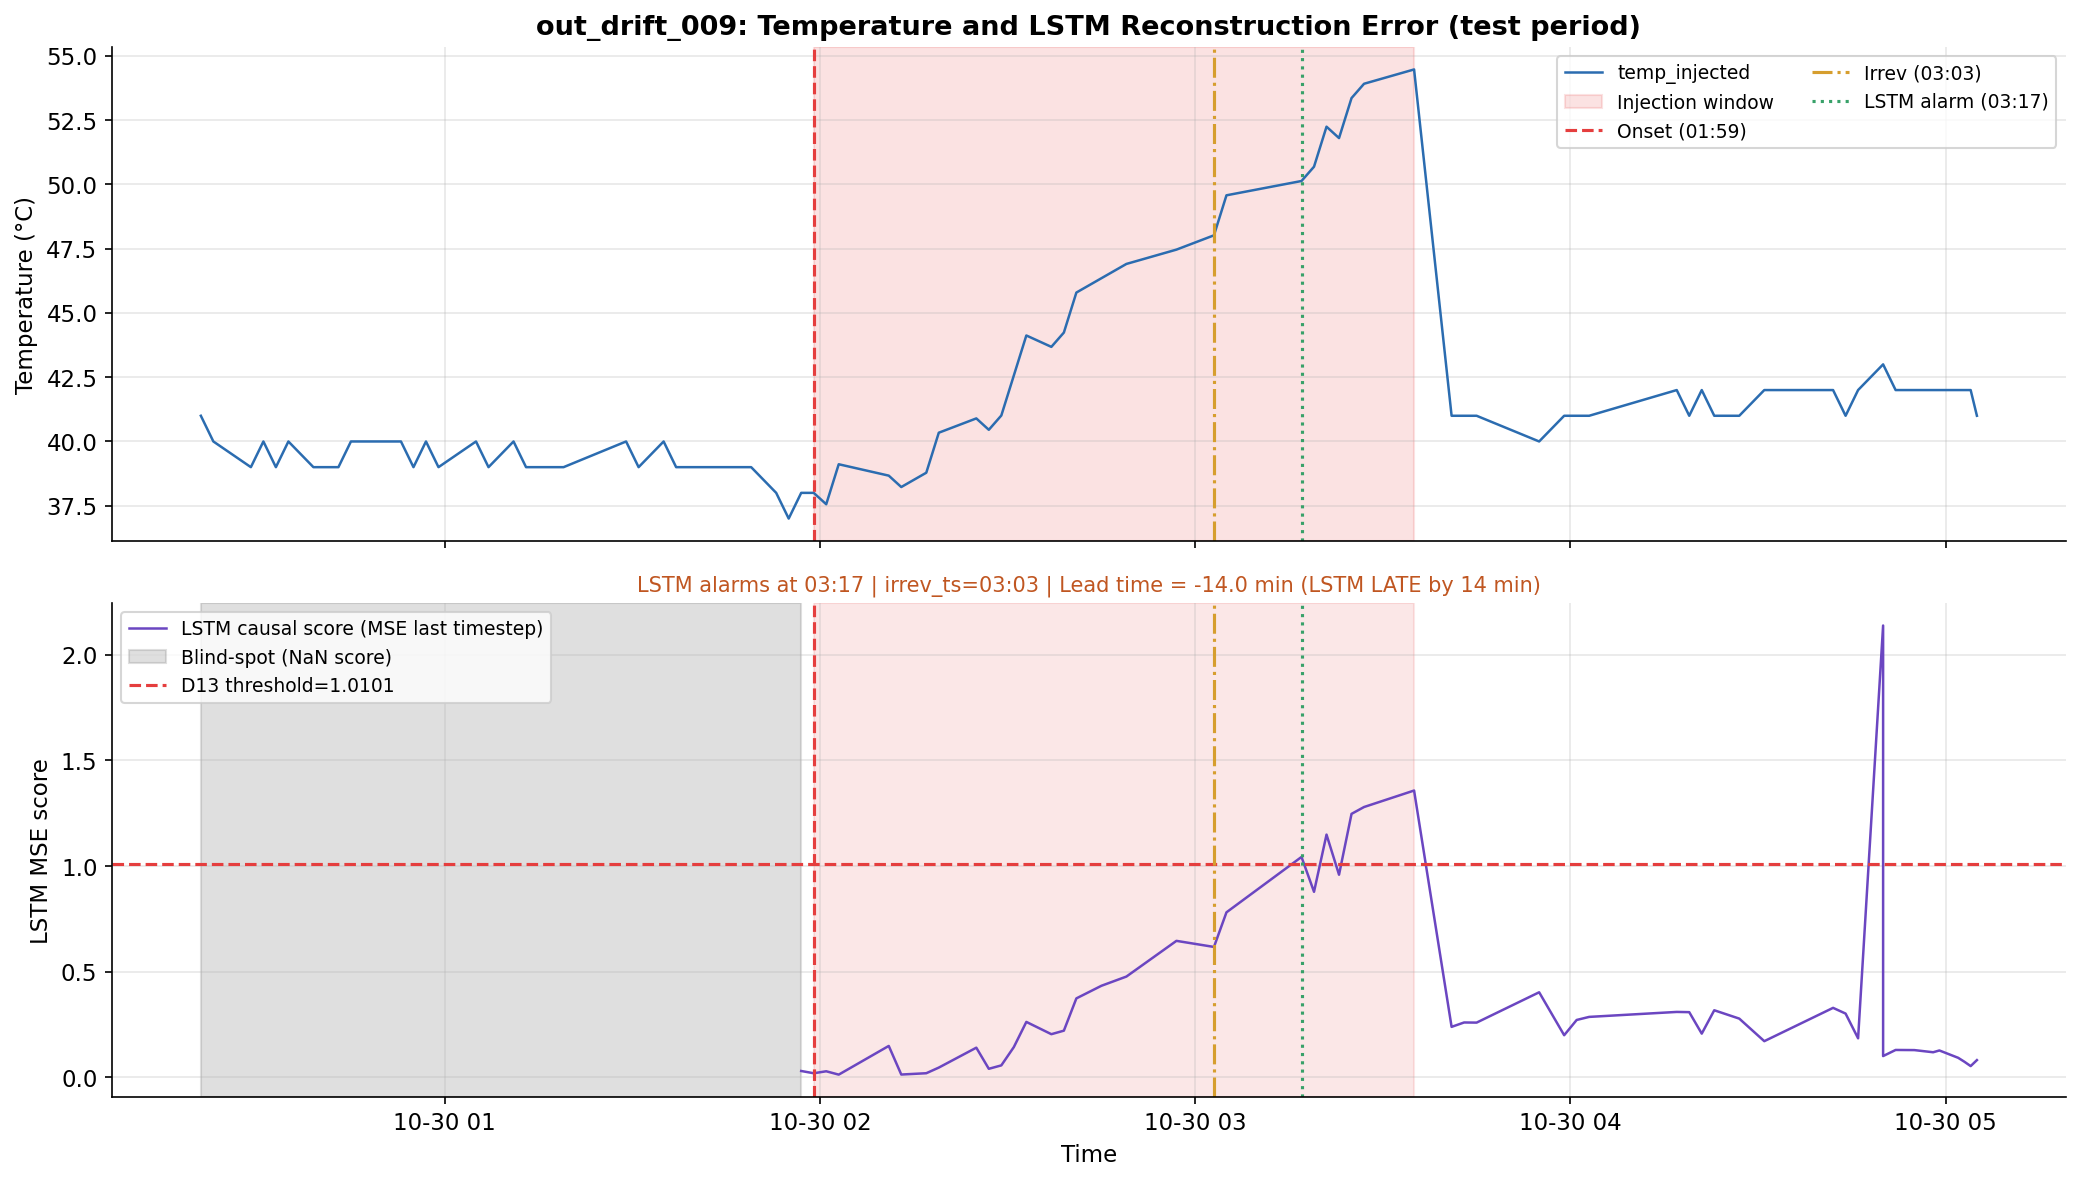
\includegraphics[width=0.92\textwidth]{figures/fig_m4b_reconstruction_error_drift.png}
    \caption{The one case where the LSTM-Autoencoder is measurably late: \texttt{out\_drift\_009}. The reconstruction-error score crosses its threshold only after irreversibility onset (14.0 minutes late), illustrating that a reconstruction-based detector can lag a fast-accelerating drift even when its score does eventually respond correctly.}
    \label{fig:reconstruction_drift}
\end{figure}

\section{Digital-Twin Replay and Cross-Check Verification}
\label{sec:res_twin}

The SimPy digital twin's replay of the real sensor stream was verified byte-exact against the source data: zero value mismatches, $0.00\times10^{0}$s simulated-time discrepancy, full replay completing in 6.03 seconds of wall-clock time. With the three live monitors (\texttt{BaselineMonitor}, \texttt{IFMonitor}, \texttt{LSTMMonitor}) wired into the Destination stage, the twin's live alerts were cross-checked row-by-row against the offline batch-evaluation results (\texttt{data/processed/twin\_crosscheck\_report.csv}, 90 rows $=$ 30 injections $\times$ 3 detectors):

\begin{keyfinding}[RQ3 Resolved: 100\% Live/Batch Parity]
Across all 30 injections and 3 detectors, 42 comparisons were scientifically applicable (all 30 baseline comparisons, plus the 6 test-side Isolation Forest and 6 test-side LSTM comparisons); every one of these 42 matched exactly (\texttt{match = True}, 0 mismatches). The remaining 48 comparisons (train-side Isolation Forest and LSTM results) are correctly excluded from performance claims and marked \texttt{not\_applicable}, retained only as demonstration material. The live digital twin and the offline batch evaluation never silently diverge.
\end{keyfinding}

% ==============================================================================
% CHAPTER 7: METHODOLOGICAL JOURNEY
% ==============================================================================
\chapter[Methodological Journey]{Methodological Journey: Key Design Decisions}
\label{chap:methodological_journey}

A primary contribution of this project is its transparent, append-only Architectural Decision (AD) log (\texttt{docs/AD\_LOG.md}, 35 formal entries spanning D1--D35), documenting every rejected assumption, caught bug, and empirical pivot rather than presenting only a clean final pipeline. Table~\ref{tab:ad_log} summarises five of the most consequential entries.

\begin{table}[H]
\centering
\caption{Summary of Methodological Design Decisions (AD Log).}
\label{tab:ad_log}
\small
\begin{tabularx}{\textwidth}{L{1.3cm} L{3.1cm} L{3.6cm} Y}
\toprule
\textbf{Decision} & \textbf{What Was Tried} & \textbf{What Was Found} & \textbf{What Was Done Instead} \\
\midrule
D1--D4 & Search for the alarm/irreversibility comparison window with no upper bound (search to end of series). & The unbounded search could pick up unrelated future events, artificially inflating lead-time claims by orders of magnitude. & Bounded the search to \texttt{SEARCH\_HORIZON\_MINUTES=60} from injection onset, giving the lead times reported in \cref{tab:leadtime}. \\
\addlinespace
D22 & Audit whether the Isolation Forest's rolling-mean/rolling-std features used a centred (\texttt{center=True}) window, which would leak future values into the current row's features. & The rolling features were confirmed genuinely causal (trailing window only), so no look-ahead leakage was present in the reported Isolation Forest results. & Retained the existing causal rolling-feature implementation; documented the audit outcome as a positive verification rather than a silent assumption. \\
\addlinespace
D17--D19 & Build the SimPy digital-twin replay engine and assume it faithfully reproduces the source stream. & Verified instead of assumed: byte-exact replay, 0 value mismatches, $0.00\times10^{0}$s simulated-time discrepancy across a full 6.03-second replay. & Proceeded to wire live detectors into the Destination stage only after this verification passed. \\
\addlinespace
D26 & Include all 30 injections' Isolation Forest/LSTM live-monitor results in headline performance claims. & 24 of the 30 injections fall on the training side of the chronological split; including them would contaminate performance claims with in-sample results. & Restricted all Isolation Forest/LSTM performance claims to the 6 test-side injections only; retained the 24 train-side comparisons as demonstration-only material, explicitly labelled as such. \\
\addlinespace
D35 & Maintain a hand-transcribed comparison table (in a results notebook) of both detectors' point-wise confusion-matrix counts, alongside a separately hand-written summary in the AD log. & The two hand-transcribed sources disagreed with each other, and the notebook table was internally arithmetically inconsistent for one column (reported FN did not reconcile with its own reported recall and true-anomaly count). & Serialized both detectors' point-wise metrics directly from the evaluation code to machine-generated JSON files, added a permanent \texttt{TP+FN == true anomalies} regression assertion, and made the notebook load the JSON live rather than maintain a parallel hardcoded copy. \\
\bottomrule
\end{tabularx}
\end{table}

\begin{methodologydecision}[D35 in Detail --- A Single-Source-of-Truth Violation]
During preparation of this report, cross-verification against the live repository revealed that a results-comparison table in \texttt{notebooks/04\_lstm\_evaluation.ipynb} reported Isolation Forest point-wise metrics that were both internally inconsistent (a reported \texttt{FN=3} did not reconcile with the same cell's reported recall of 0.8000 and true-anomaly count of 65, which together imply $\text{FN}=13$) and materially different from the corresponding entry already recorded in the AD log (D7). Neither hand-transcribed source was backed by a machine-generated, reproducible artefact. Re-running the evaluation pipeline end-to-end with a newly added \texttt{TP+FN} consistency assertion confirmed that the AD log's originally recorded figures were the accurate ones, and that the notebook table's Isolation Forest columns had been transcribed from a stale or incorrect intermediate run. The fix was verified via a fresh clone of the repository at the resulting commit: the corrected JSON artefacts, the updated notebook cell (now loading those JSON files live instead of a hardcoded dictionary), and an append-only new AD log entry were all confirmed byte-for-byte, with every protected file (README, dashboard, LSTM model weights, the lead-time comparison table, and every pre-existing AD log entry D1--D34) confirmed completely unchanged by \texttt{git diff}.
\end{methodologydecision}

% ==============================================================================
% CHAPTER 8: INTERACTIVE DIGITAL TWIN DASHBOARD
% ==============================================================================
\chapter[Digital Twin Dashboard]{Interactive Digital Twin Dashboard}
\label{chap:dashboard}

To make the digital twin's live behaviour directly inspectable rather than only reportable as static tables, the complete pipeline is deployed as a public, interactive Streamlit web application:

\begin{center}
\url{https://coldchain-ews-twin.streamlit.app/}
\end{center}

\begin{limitationbox}[Screenshots Pending]
This chapter describes the dashboard's verified, documented behaviour (\texttt{dashboard/README.md}) in full, but does not yet include screenshots of the live interface. Screenshots will be added once supplied, so that this chapter's figures are genuine captures of the deployed application rather than an artist's impression of it.
\end{limitationbox}

\section{Zero-Duplication Architecture}
\label{sec:dash_architecture}

The dashboard imports \texttt{BaselineMonitor}, \texttt{IFMonitor}, and \texttt{LSTMMonitor} directly from \texttt{src/twin\_monitors.py}, and the same stable event-sorting logic from \texttt{src/digital\_twin.py} (AD Log D27): no detection logic is re-implemented for presentation purposes, so the dashboard cannot silently drift from the verified pipeline described in \cref{chap:methodology}. A startup verification gate (D32) checks for the presence of all seven required model and data artefacts before permitting any playback, halting with explicit remediation instructions if any are missing.

\section{Operating Modes}
\label{sec:dash_modes}

\textbf{Guided Tour} presents a curated four-step sequence across the six test-side injections, built specifically for viva-style walkthroughs: the abrupt step injection (\texttt{out\_step\_001}), where all three detectors trigger synchronously at the same reading with identical zero lead time; the incipient Out-series drift (\texttt{out\_drift\_009}), where Isolation Forest's +64.0-minute early warning and the LSTM-Autoencoder's $-$14.0-minute lag are shown side by side; the in-range sensor flatline (\texttt{out\_flatline\_013}), where the naive baseline fails to alarm at all while Isolation Forest still detects a collapse in rolling variance; and the inbound drift (\texttt{in\_drift\_023}), where Isolation Forest's +11.0-minute early warning is contrasted with the baseline and LSTM triggering only at threshold crossing.

\textbf{Free Explore} allows inspection of all 30 synthetic injections across both series, with every injection explicitly tagged \texttt{[TEST]} (scientifically valid, out-of-sample) or \texttt{[TRAIN\allowbreak\ DEMO]} (training-region preview only, no performance claim made) -- directly surfacing the same train/test discipline enforced throughout the batch evaluation (AD Log D26, D31).

\section{Replay Fidelity Safeguards}
\label{sec:dash_fidelity}

Playback speed (1$\times$ through Instant) is purely a UI rendering choice: the telemetry values, gaps, and timestamps actually passed to the detectors are identical regardless of display speed (AD Log D28). A silent buffer pre-warming step (AD Log D33) primes the Isolation Forest's 10-reading rolling buffer and the LSTM's 30-reading window buffer with the preceding readings \emph{before} the visible playback window begins, eliminating cold-start artefacts; this was verified to produce an exact 18/18 alarm match against the batch pipeline (\texttt{tests/test\_d33\_prewarm.py}). All narrative captions are interpolated at runtime directly from \texttt{three\_way\_comparison.csv} and \texttt{twin\_crosscheck\_report.csv} (AD Log D34) rather than hardcoded, so the dashboard's displayed numbers cannot silently drift out of sync with the underlying evaluation data.

% ==============================================================================
% CHAPTER 9: DISCUSSION
% ==============================================================================
\chapter{Discussion}
\label{chap:discussion}

The experimental findings directly resolve the three research questions posed in \cref{sec:rqs}:

\begin{enumerate}[leftmargin=*,itemsep=6pt]
    \item \textbf{Resolution of RQ1 (Early-Warning Lead Time):} An anomaly-detection model embedded in the digital twin \emph{can} flag a disruption meaningfully earlier than a fixed-threshold alarm, but only for the gradual, drift-type disruption category, and only using the classical Isolation Forest detector: +64.0 minutes on the Out series and +11.0 minutes on the In series. This is consistent, in order of magnitude, with the maritime-refrigerated-container literature's reported median lead time of approximately 68 minutes for an analogous hybrid digital-twin/deep-learning detector \parencite{vuksic2026early}, lending independent plausibility to the general claim that reconstruction- or isolation-based scores can out-run a threshold alarm on gradual disruptions by tens of minutes. For abrupt, step-type disruptions, all three detectors trigger at the identical timestamp, because a sufficiently large instantaneous jump crosses every detector's decision boundary simultaneously -- there is no early-warning advantage to be had when the anomaly is not itself a slow-building precursor. For flatline disruptions, neither detector improves on the (non-firing) baseline in a lead-time sense, because a flatline that never crosses the fixed threshold never generates an irreversibility timestamp against which lead time can even be measured.

    \item \textbf{Resolution of RQ2 (Classical vs.\ Deep-Learning Trade-offs):} Neither detector dominates the other. Isolation Forest wins on drift-type lead time and on point-wise recall on both series, at the cost of a high false-positive rate (\cref{tab:pointwise}). The LSTM-Autoencoder is markedly more conservative and precision-favouring specifically on the In series (13.1\% precision, 2.9\% FPR, AUC-PR 0.385 -- its best result by a wide margin), but is measurably \emph{late} on the one Out-series drift case where lead time can be computed, and its Out-series point-wise AUC-PR (0.0049) is close to chance. This asymmetry -- strong on In, weak on Out -- is plausibly linked to the In series' shorter length (20,345 vs.\ 77,261 raw readings) and different sampling characteristics; the LSTM had less In-series data to learn a reconstruction manifold from, yet performed better there point-wise, suggesting the Out series' greater volume did not translate into a proportionally better learned representation, an open question for future work rather than one this project can resolve with the data at hand.

    \item \textbf{Resolution of RQ3 (Live Digital-Twin Fidelity):} The 100\% exact match between the live SimPy digital twin and the offline batch evaluation (\cref{sec:res_twin}) confirms that embedding a model as a live monitor inside a discrete-event simulation, rather than running it as a one-shot batch script, introduces no silent discrepancy in this implementation -- provided the buffer pre-warming safeguard (AD Log D33) is in place to eliminate cold-start artefacts at the start of any windowed playback.
\end{enumerate}

\textbf{On the point-wise metrics gap versus domain-specific literature:} \textcite{xie2025anomaly}'s improved Isolation Forest reports F1 scores around 0.86 on real cold-chain-logistics fleet data, dramatically higher than this project's own Isolation Forest F1 (0.017 Out, 0.040 In). This gap is a direct consequence of task structure rather than a modelling failure: their evaluation labels naturally occurring environment/node/measurement anomalies across five co-located sensor modalities per vehicle node, producing a comparatively balanced anomaly prevalence, whereas this project's point-wise metrics are computed against a deliberately sparse set of synthetically injected single-channel events (65 true-anomaly rows out of 13,372 test rows on the Out series, a prevalence of roughly 0.5\%) inside a single-sensor univariate stream. A precision-recall curve is fundamentally limited by class prevalence, and this project's honest, low-prevalence, single-channel injection design was chosen specifically to avoid overstating anomaly frequency; the resulting low absolute F1 scores are an expected consequence of that choice, not evidence that the underlying detectors are poorly implemented -- a distinction made explicit here rather than left for the reader to reconstruct.

% ==============================================================================
% CHAPTER 10: SCOPE AND LIMITATIONS
% ==============================================================================
\chapter{Scope and Limitations}
\label{chap:limitations}

To maintain research credibility, the boundaries of this study are explicitly documented:

\begin{limitationbox}[Summary of Project Scope and Constraints]
\begin{itemize}[leftmargin=*,itemsep=4pt]
    \item \textbf{Structural-Proxy Dataset, Not Real Cold-Chain Telemetry:} The Kaggle IoT temperature stream has no real multi-sensor spatial topology, no refrigeration-range temperatures, and no ground-truth disruption labels. Every quantitative result in this report describes performance on this proxy construct.
    \item \textbf{No Real-World Validation:} All anomalies evaluated are synthetically injected and explicitly labelled as such; no real cold-chain disruption event, of any kind, has been detected or claimed to be detected by this system.
    \item \textbf{Sparse, Single-Channel Injection Design:} The injection protocol seeds anomalies into a single temperature channel per series at a deliberately low prevalence, which structurally limits point-wise precision/recall/F1 relative to richer, multi-sensor, higher-prevalence real-world benchmarks (\cref{chap:discussion}).
    \item \textbf{Small Test-Side Injection Count:} Only 6 injections are available for scientifically valid lead-time claims (2 per anomaly type, split across 2 series minus one missing In-flatline test case), which is sufficient to reveal a genuinely mixed result but not sufficient to support strong statistical generalisation claims about detector performance across anomaly types.
    \item \textbf{No Physical Thermal Model:} Unlike hybrid physics-based digital twins in the maritime cold-chain literature \parencite{vuksic2026early}, this project's digital twin is a pure data-pipeline replay (Source $\rightarrow$ Transit $\rightarrow$ Destination) with no underlying physical thermal or refrigeration model; it is a proxy for the data-flow architecture of a cold-chain monitoring system, not for its physical dynamics.
    \item \textbf{GPU-Constrained Architecture:} The LSTM-Autoencoder was deliberately kept small enough to train on a free-tier Google Colab T4 GPU session; a larger architecture, trained on more powerful hardware, might narrow or reverse the Out-series performance gap reported in \cref{sec:res_pointwise}, but this was explicitly out of scope for this project.
\end{itemize}
\end{limitationbox}

% ==============================================================================
% CHAPTER 11: CONCLUSION AND FUTURE WORK
% ==============================================================================
\chapter{Conclusion and Future Work}
\label{chap:conclusion}

\section{Conclusion}
\label{sec:conclusion}

This project developed, empirically tested, and publicly deployed a digital-twin-integrated early-warning system for cold-chain disruption detection, built entirely from open-source tools and a transparently labelled structural-proxy IoT dataset in place of unavailable real cold-chain telemetry. Wiring an Isolation Forest baseline and an LSTM-Autoencoder into a SimPy discrete-event digital twin, and cross-checking the twin's live output against an independent offline batch evaluation, produced a 100\% exact match across all 30 synthetic injections and 3 detectors -- directly answering whether a live-embedded model can silently diverge from its offline counterpart (it does not, given adequate buffer pre-warming).

On the six scientifically valid test-side injections, Isolation Forest delivered a genuine early-warning advantage over a naive fixed-threshold baseline on both drift-type disruptions (+64.0 and +11.0 minutes), while the LSTM-Autoencoder was measurably late on the one case where a direct comparison was possible. Point-wise classification metrics revealed a further, independent trade-off: Isolation Forest's high recall came with a high false-positive rate, while the LSTM-Autoencoder's markedly better In-series precision came with weak Out-series detection. Both results are reported exactly as measured, including the LSTM's underperformance, in keeping with a zero-fabrication, evidence-first standard maintained throughout via a 35-entry append-only Architectural Decision log -- a log that itself caught and corrected two genuine methodological errors during the project's own development: an originally unbounded lead-time search window, and a hand-transcribed results table that disagreed with, and was ultimately shown to be wrong relative to, the pipeline's own live-computed metrics.

\section{Future Research Directions}
\label{sec:future_work}

\begin{enumerate}[leftmargin=*,itemsep=4pt]
    \item \textbf{Real Cold-Chain Telemetry Validation:} Partnering with a cold-chain logistics operator to obtain real, ideally labelled, refrigerated-transport sensor data would allow this pipeline's methodology to be re-run on genuine cold-chain telemetry rather than a structural proxy, directly testing whether the findings in \cref{chap:results} transfer.
    \item \textbf{Richer, Multi-Sensor Injection Design:} Extending the injection protocol to multiple co-located sensor channels (temperature, humidity, door-open events) per node, as in \textcite{xie2025anomaly}, would allow point-wise metrics to be benchmarked on a more favourable, higher-prevalence footing directly comparable to domain-specific literature.
    \item \textbf{Hybrid Physics-Informed Digital Twin:} Incorporating a lightweight physical thermal model into the digital twin's Source or Transit stage, in the style of \textcite{vuksic2026early}, would allow physically interpretable residuals to be fused with the existing learned anomaly scores, potentially narrowing the LSTM-Autoencoder's Out-series performance gap.
    \item \textbf{Larger-Scale LSTM Architectures:} Relaxing the free-tier Colab T4 GPU constraint to test whether a larger LSTM-Autoencoder narrows or reverses the Out-series underperformance identified in \cref{chap:discussion}.
    \item \textbf{Expanded Test-Side Injection Count:} Seeding a larger number of test-side injections per anomaly type would allow the genuinely mixed result in \cref{sec:res_leadtime} to be assessed with formal statistical significance testing, which the current 6-injection test set is too small to support.
\end{enumerate}

% ==============================================================================
% CHAPTER 12: CONTRIBUTION AND VALUE
% ==============================================================================
\chapter{Contribution and Value}
\label{chap:contribution}

\begin{itemize}[leftmargin=*,itemsep=5pt]
    \item \textbf{Technical Contribution:} An end-to-end, reproducible integration architecture bridging classical anomaly detection (Isolation Forest), deep-learning reconstruction-based anomaly detection (LSTM-Autoencoder), and discrete-event digital-twin simulation (SimPy), with a live/batch cross-check verifying zero silent divergence between the two.
    \item \textbf{Methodological Contribution:} A transparently documented protocol for building and evaluating a cold-chain-adjacent anomaly-detection system entirely from openly available data, using explicit structural-proxy labelling and a chronologically disciplined synthetic-injection design in place of unavailable real disruption labels -- directly addressing the proprietary-data gap identified in \cref{chap:research_gap}.
    \item \textbf{Practical Contribution:} A publicly accessible, interactive Streamlit dashboard allowing direct inspection of the digital twin's live detector behaviour, curated for viva-style walkthroughs via a Guided Tour mode and open-ended inspection via a Free Explore mode.
    \item \textbf{Corporate Entrepreneurship Value:} A tangible demonstration of disciplined, evidence-first decision-making under data scarcity and uncertainty -- exemplifying how a technology-adoption decision should be evaluated by validating assumptions, auditing evaluation pipelines for silent errors, and reporting mixed or unfavourable results exactly as measured, rather than presenting only a convenient subset of the evidence.
\end{itemize}

% ==============================================================================
% REFERENCES
% ==============================================================================
\clearpage
\printbibliography[heading=bibintoc,title={References}]

% ==============================================================================
% APPENDICES
% ==============================================================================
\appendix

% ------------------------------------------------------------------------------
% APPENDIX A: TECHNOLOGY STACK
% ------------------------------------------------------------------------------
\chapter{Technology Stack}
\label{chap:tech_stack}

\begin{table}[H]
\centering
\caption{Project Technology Stack and Dependency Specifications.}
\label{tab:tech_stack}
\small
\begin{tabularx}{\textwidth}{L{3.2cm} L{3.6cm} Y}
\toprule
\textbf{Component Layer} & \textbf{Libraries / Frameworks} & \textbf{Functionality in Project} \\
\midrule
Core Programming & Python, NumPy, Pandas & Core numerical arrays, tabular transformations, and chronological data handling. \\
Machine Learning & Scikit-Learn ($\geq$1.3.0), joblib & Isolation Forest anomaly detector, model persistence. \\
Deep Learning & TensorFlow ($\geq$2.15.0) & LSTM-Autoencoder architecture, training on Google Colab T4 GPU, CPU inference. \\
Discrete-Event Simulation & SimPy ($\geq$4.1.0) & Three-stage (Source $\rightarrow$ Transit $\rightarrow$ Destination) digital-twin replay engine. \\
Visualization & Matplotlib ($\geq$3.8.0), Seaborn ($\geq$0.13.0) & Precision-recall curves, reconstruction-error timelines, and lead-time comparison charts. \\
Interactive Dashboard & Streamlit ($\geq$1.33.0), Altair ($\geq$5.0.0) & Reactive web UI, Guided Tour and Free Explore playback modes. \\
Data Acquisition & kagglehub, kaggle & Programmatic download of the structural-proxy IoT telemetry dataset. \\
Notebooks \& Testing & Jupyter, nbformat, nbclient, nbconvert, ruff & Milestone notebooks (01--06), code-quality linting, and the D33 buffer pre-warming regression test. \\
\bottomrule
\end{tabularx}
\end{table}

% ------------------------------------------------------------------------------
% APPENDIX B: REPRODUCTION INSTRUCTIONS
% ------------------------------------------------------------------------------
\chapter[Reproduction Instructions]{Repository and Reproduction Instructions}
\label{chap:reproduction}

The complete source code, evaluation pipeline, Architectural Decision log, and dashboard application are version-controlled and publicly accessible:

\begin{center}
\textbf{GitHub Repository:} \url{https://github.com/Krishna200608/coldchain-ews-twin}
\end{center}

\section{Environment Setup and Pipeline Execution}
\label{sec:reproduction}

To reproduce the full pipeline from scratch:

\begin{enumerate}[leftmargin=*,itemsep=3pt]
\item \textbf{Clone Repository and Install Dependencies:}
\begin{verbatim}
git clone https://github.com/Krishna200608/coldchain-ews-twin.git
cd coldchain-ews-twin
python -m venv .venv
source .venv/bin/activate
# Windows: .\.venv\Scripts\activate
pip install -r requirements.txt
\end{verbatim}

\item \textbf{Execute Data Acquisition, Injection, and Baseline Pipeline:}
\begin{verbatim}
python src/data_acquisition.py
python src/preprocessing.py
python src/anomaly_injection.py
python src/baseline_and_labels.py
\end{verbatim}

\item \textbf{Train and Evaluate Isolation Forest:}
\begin{verbatim}
python src/isolation_forest_model.py
python src/if_evaluation.py
\end{verbatim}

\item \textbf{Prepare LSTM Windows, Train on Colab T4 (see \texttt{colab/\allowbreak lstm\_train.ipynb}), then Evaluate:}
\begin{verbatim}
python src/lstm_prep.py
# Train on Colab (T4 GPU), then pull models/lstm_{out,in}.h5
python src/lstm_evaluation.py
\end{verbatim}

\item \textbf{Run the Digital-Twin Replay and Cross-Check:}
\begin{verbatim}
python src/twin_monitors.py
python src/twin_crosscheck.py
\end{verbatim}

\item \textbf{Run the Test Suite:}
\begin{verbatim}
pytest tests/ -v
\end{verbatim}

\item \textbf{Launch the Interactive Local Dashboard:}
\begin{verbatim}
streamlit run dashboard/app.py
\end{verbatim}
\end{enumerate}

\end{document}
